% Repository:  https://github.com/chiehrosswang/TRB_LaTeX_tex
%
% Transportation Research Board conference paper template
% version 4.0 Lite (updates made to be compatible in Overleaf and ShareLaTeX)
%
%
% When numbered option is activated, lines are numbered.
\documentclass[]{trbunofficial}
\usepackage{graphicx}
\usepackage{booktabs}

\newread\somefile
\usepackage{xparse}
\usepackage{natbib}
\bibliographystyle{unsrtnat}
\setcitestyle{round}
% \usepackage[colorlinks=true,linkcolor=blue,citecolor=blue]{hyperref}
% For TRB version hide links
\usepackage[hidelinks]{hyperref}

% Put here what will go to headers as author
\AuthorHeaders{}
\title{Competition for Access to Opportunities between Modes: Multimodal
Spatial Availability}

% TODO: add macros for easier formatting of \author.
\author{%
    \textbf{Anastasia Soukhov}\\\textit{Corresponding Author}\\
  PhD Candidate\\
  Department of Earth, Environment and Society, McMaster University,
Canada\\
  \href{mailto:soukhoa@mcmaster.ca}{\nolinkurl{soukhoa@mcmaster.ca}}\\
  \hfill\break
    \textbf{Javier Tarriño-Ortiz}\\
  PhD Graduate\\
  Universidad Politécnica de Madrid, Spain\\
  \href{mailto:javier.tarrino.ortiz@upm.es}{\nolinkurl{javier.tarrino.ortiz@upm.es}}\\
  \hfill\break
    \textbf{Julio A. Soria-Lara}\\
  Associate Professor\\
  Urban and Regional Planning, Universidad Politécnica de Madrid,
Spain\\
  \href{mailto:julio.soria-lara@upm.es}{\nolinkurl{julio.soria-lara@upm.es}}\\
  \hfill\break
    \textbf{Antonio Páez}\\
  Associate Professor\\
  Department of Earth, Environment and Society, McMaster University,
Canada\\
  \href{mailto:paezha@mcmaster.ca}{\nolinkurl{paezha@mcmaster.ca}}\\
  \hfill\break
  }

% If necessary modify the number of words per table or figure default is set to
% 250 words per table (default defined in cls)


% If words are counted manually, put that number here. This does not include
% figures and tables. This can also be used to avoid problems with texcount
% program i.e. if one does not have it installed.
\TotalWords{7195}


% tightlist command for lists without linebreak
\providecommand{\tightlist}{%
  \setlength{\itemsep}{0pt}\setlength{\parskip}{0pt}}



\usepackage{multirow}
\usepackage{multicol}
\usepackage{colortbl}
\usepackage{hhline}
\newlength\Oldarrayrulewidth
\newlength\Oldtabcolsep
\usepackage{longtable}
\usepackage{array}
\usepackage{hyperref}
\usepackage{float}
\usepackage{wrapfig}

\begin{document}
\maketitle


\section{Abstract}
An increasing number of studies within the domain of transportation
planning are concerned with the inequities in accessibility to
opportunities. A dimension of these inequities arises from differences
in access by mode type (e.g., commuting using a car as opposed to
transit). However, methods implemented in current accessibility
literature are lacking within the context of multimodal analysis. This
paper presents an extension of spatial availability, a
singly-constrained competitive accessibility measure, for the context of
multimodal accessibility analysis. We first illustrate the features of
spatial availability that lend itself to multimodal analysis. We then
demonstrate its use on the case study of Low Emission Zones in Madrid
(Spain) and highlight how this policy intervention changes the
accessibility of populations using different modes. In summary, spatial
availability can be used to create and interpret multimodal policy
intervention scenarios unlike previous methods: this creation and
interpretation can help regions envision a more sustainable and
equitable access-to-opportunity landscape.
\hfill\break%
\hfill\break%
\noindent\textit{Keywords}:  Multimodal, Accessibility, Equity, Policy
scenarios, Low emission zones,  
\newpage

\hypertarget{abstract}{%
\section{Abstract}\label{abstract}}

An increasing number of studies within the domain of transport are
concerned with the inequities in accessibility to opportunities. A
dimension of these inequities arise from differences in access by mode
type (e.g., the number of work opportunities that can be reached using a
car as opposed to transit in a city). However, methods assessing
multimodal accessibility in the literature fall short as aspects of
competition for opportunities and the explicit methodological
acknowledgement of opportunities being \emph{finite} are lacking. In
this vein, this paper presents an extension of \emph{spatial
availability}, a singly-constrained competitive accessibility measure,
for the context of multimodal accessibility analysis. We first
illustrate the features of spatial availability that lends itself to
multimodal analysis. We then demonstrate its use on the case study of
Low Emission Zones in Madrid (Spain) and highlight how this policy
intervention changes the accessibility of populations using different
modes. In summary, spatial availability can be used to create and
interpret multimodal policy intervention scenarios unlike previous
methods: this creation and interpretation can help regions envision a
more sustainable and equitable access-to-opportunity landscape by better
identifying differences in accessibility afforded by different modes.

\hypertarget{introduction}{%
\section{Introduction}\label{introduction}}

Implementing urban policies that re-shape cities through accessibility
gains (i.e., the \emph{potential to interact} with opportunities as a
result of land-use mix and transport systems as originally defined by
\citet{hansenHowAccessibilityShapes1959}) have been widely applied
within the transportation literature and is increasingly discussed by
planners
\citep{levinsonTransportAccessManual2020, gowerPlanningInnovationCity2022, siddiqToolsTradeAssessing2021, yanAccessibilityBasedPlanningAddressing2021}.
An important challenge in the identification of interventions that
equitably transform cities is the effective evaluation of
\emph{trade-offs}: cities are complex and dynamic ecologies, and
advantaging one component of the city can disadvantage another area,
population, or sub-component In this way, policy evaluation should take
a \emph{systems} approach
\citep{fikselSustainabilityResilienceSystems2006}. One way of
considering systems is from the perspective of the \emph{finite}. As an
illustration, consider the amount of transport space within a city: the
amount is typically finite so re-allocating road space away from one
mode directly impacts the performance of the others (see the literature
on road space reallocation e.g.,
\citet{valencaMainChallengesOpportunities2021}). Evaluating policy
impacts in the context of \emph{finity} provides a way to contextualize
the balance of trade-offs that the citizens of a city should tolerate.

From the perspective of urban transport systems, location-based
accessibility measures have been used in the context of policy
evaluation. For instance, \citet{leeMeasuringImpactsNew2018} assesses
the transit accessibility gains to healthcare and employment
opportunities for disadvantaged neighbourhood in Columbus, Ohio, USA
after the transit system's re-design and introduction of a rapid bus
system. However, a limitation of this study, like others that implement
accessibility measures, is they do not calculate results under a
\emph{constrained} framework i.e., one of \emph{finity}. The citizens of
Columbus should experience qualitative accessibility gains - but is it
at the expense of access to opportunities to populations using other
modes?

The work of \citet{leeMeasuringImpactsNew2018} uses
\emph{non-competitive} accessibility measures. There is a branch of
location-based accessibility measures that do incorporate the effect of
competition for opportunities by the population in the region. However,
we argue that these existing methods fall short in acknowledging the
\emph{finity} of opportunities. For instance,
\citet{maoMeasuringSpatialAccessibility2013} applies a competitive
measure, two-step floating catchment approach (2SFCA), for the case of
access to healthcare services in Florida for both a multimodal network
and a single modal network. While the differences in modal access are
discussed, the question of how the advantage in access afforded by one
mode over another impacts access for different mode users is unanswered.

This question of how much one mode-using population can access at the
expense of another mode-using population is a pertinent equity question
in the evaluation of policy scenarios that are multimodal. For instance,
consider the impact of a low emission zone (LEZ). LEZ is a policy of
spatial and modal discrimination: the circulation of vehicles that are
excessively polluting are restricted in specific regions. In the
recognition that opportunities are finite, the implementation of a LEZ
explicitly reduces the access that the population using polluting
vehicles has to opportunities. This restriction allows the population
using other more sustainable modes to potentially have a higher level of
access than before the LEZ implementation. This evaluation is especially
urgent as LEZ are currently in effect in cities globally; their
reception has been mixed \citep{tarrinoortizPublicAcceptabilityLow2021}
and may be having negative impacts on disadvantaged populations who have
become mobility restricted
\citep{devrijNooneVisitsMe2022, verbeekJustManagementUrban2022}.
Measures that evaluate the accessibility of modes given both
\emph{constrained} and \emph{competitive} considerations are lacking in
the literature, but are needed, to evaluate such policy interventions
impact on accessibility.

In \citet{soukhovIntroducingSpatialAvailability2023}, we introduce
spatial availability, a type of location-based accessibility measure
that is both \emph{constrained} and \emph{competitive}. In this paper,
we extend the spatial availability measure into a multimodal framework
and explore its use in answering the question outlined: \emph{``given
opportunities are finite, how many are available to a given location
depending on the mode used?''.} The answer to this question quantifies
how many opportunities can be accessed, considering competition, for
different modes. To foreground this exploration, in Section 2, we
discuss short falls of a few existing location-based measures in
comparison to spatial availability through a synthetic example. In
Section 3, the spatial availability of an empirical example of the LEZ
in the city of Madrid, Spain is calculated. We demonstrate how the
restriction of car circulation could have impacted the spatial
availability of opportunities for each sub-population using transit,
cycling and walking modes. In Section 4, we provide concluding remarks
on the strengths of the use of spatial availability as a multimodal
accessibility measure and potential future uses in policy planning
scenarios.

\hypertarget{a-review-of-multimodal-accessibility-measures}{%
\section{A review of multimodal accessibility
measures}\label{a-review-of-multimodal-accessibility-measures}}

Location-based accessibility indicators are quantitative measures of
\emph{potential} interaction with opportunities for locations within a
given region: they are a product of the relationship between land-use
and transport systems. Arguably the most commonly used location-based
measured are cumulative opportunity measures and weighted cumulative
opportunity measures \citep{levinsonTransportAccessManual2020}. These
measures weight the opportunities that can be potentially interacted
with from origin \(i\) to destination \(j\) based on some sort of travel
cost function (e.g., travel time, fare, travel distance) otherwise known
as a travel impedance function \(f^{m}(c^m_{ij})\). Many weighted
cumulative opportunities (often refered to as the gravity-based measure)
originate from the measure proposed by
\citet{hansenHowAccessibilityShapes1959}, which can take the following
multimodal form: \(S_i^m = \sum_j O_j f^m(c_{ij}^m)\) where \(m\) is a
set of modes which have mode-specific travel costs \((c_{ij}^m)\) and
travel impedance functions \(f^m(\cdot)\).

The Hansen-type measure does not consider competition between modes nor
is it constrained. As an example, the work of
\citet{tahmasbiMultimodalAccessibilitybasedEquity2019} uses the
Hansen-type measure to measure the potential interaction with retail
locations using walking, public transit, and car modes \(m\). \(S_i^m\)
is the sum of retail locations \(j\) that can potentially be interacted
with under the travel impedance as calculated for each \(i\) and \(m\).
In other words, each \(i\) has three \(S_i\) values, one per \(m\). In
this work, they demonstrate that the car mode has the highest
\(S_i^{m=car}\) values in the majority of \(i\), i.e., populations using
a car can potentially interact with the most retail opportunities than
populations using other modes. However, the higher \(S_i^{m=car}\)
values are not a result of lower \(S_i^{m}\) values for other modes: it
is not assumed that car-using populations potentially accessing more
opportunities take away potential opportunities for other populations
within the measure (no consideration for competition). This measure is
also not constrained: there is no global maximum for \(S_i\) or
\(S_i^m\) values, they are presented as a population normalized
accessibility index. This makes the interpretation of the `potentially
interacted opportunities' relative to the region, making comparisons of
the results across different regions challenging.

However, opportunities in a region can be considered finite. There are
only so many school-seats, hospital capacity, jobs, etc., in a region
and if one person interacts with an opportunity at a given time, it is
taken. As such, if one person is advantaged and has the ability to reach
more opportunities through a lower travel-cost mode, than they have more
opportunities to potentially interact with more opportunities than other
people. From the other perspective, their are fewer opportunities left
to be potentially interacted with for populations using higher
travel-cost modes. In this way, populations using modes with a higher
travel impedance are at a higher access disadvantage than populations
using lower travel impedance modes. This recognition is the motivation
behind integrating \emph{competition} for opportunities within
multimodal accessibility measures. Arguably one of the most popular
competitive location-based accessibility measures is the two-step
floating catchment area (2SFCA) approach popularized by
\citet{luoMeasuresSpatialAccessibility2003} who simplified the approach
proposed by \citet{shenLocationCharacteristicsInnercity1998} (with
similar considerations for competition in
\citet{weibullAxiomaticApproachMeasurement1976} and
\citet{josephMeasuringPotentialPhysical1982}).

The Shen-type accessibility measure's formulation is:
\(a_i^m = \sum_j \frac{O_jf^m(c_{ij}^m)}{\sum_m D_j^m}\) where \(D_j^m\)
is the potential demand for opportunities equal to travel impedance
weighted population \(\sum_i P_i^m f^m(c_{ij}^m)\). In this way, the
Shen-type measure can be understood as a ratio of the potential
opportunity supply over the potential demand for opportunities. The
measure considers competition, but it is \emph{non-constrained}. A score
of competitive potential accessibility associated is associated with
each location \(i\) for each mode \(m\), but there are no global
maximums. In other words, it is difficult to interpret the meaning of
differences in Shen-type accessibility scores between modes.

To illustrate, \citet{taoInvestigatingImpactsPublic2020a} calculates
\(a_i^m\) to jobs for different income-group populations in Shenzhen
(China) using \(m = \text{public transit}\) and \(m={car}\). They
demonstrate that \(i\) with low-income populations have lower \(a_i^m\)
than \(i\) with higher-income populations. Further, they demonstrate
that \(a_i^{m=\text{public transit}}\) is lower than
\(a_i^{m=\text{car}}\) at many \(i\), arguing that this may put \(i\)
with lower-income populations in a further disadvantage. \(a_i\) and/or
\(a_i^m\) are used to compare relative spatial differences in overall
competitive accessibility and modal competitive accessibility, but
because there is no global maximum, making it is difficult to interpret
the significance between differences in \(a_i^{m}\) values. Questions
such as: what is the impact that competition has on the difference in
\(a_i^m\) values? How does impact vary spatially? And what is the
interpretation of this difference? are left unanswered.

Spatial availability improves on previous multimodal accessibility
approaches as it considers \emph{competition} in the potential
interaction with opportunities in a \emph{constrained} framework (e.g.,
finite opportunities). This is done by considering: 1) competition
between mass effect (e.g., the advantage of sub-populations residing in
relatively low population-density and high opportunity-proximate areas)
and 2) competition between travel impedance (e.g., sub-populations with
relatively low travel-impedance) through a proportional allocation
mechanism. The following sub-section demonstrates how spatial
availability compares to the Hansen-type and Shen-type measures through
a synthetic example.

\hypertarget{multimodal-spatial-availability-v_im}{%
\subsection{\texorpdfstring{Multimodal spatial availability
\(V_i^m\)}{Multimodal spatial availability V\_i\^{}m}}\label{multimodal-spatial-availability-v_im}}

In brief, we define the \emph{spatial availability} at \(i\) ( \(V_{i}\)
) as the proportion of all opportunities in the region \(O\) that are
allocated to location \(i\) from all opportunity destinations \(j\).
\(V_{i}\) is a value of how many opportunities are available to each
location \(i\) out of all the opportunities in the region. The general
formulation of spatial availability \(V_{i}\) is shown in Equation
(\ref{eq:spatial-availability-general}):

\begin{equation}
\label{eq:spatial-availability-general}
V_i = \sum_{j=1}^J O_jF^t_{ij}
\end{equation}

\noindent Where:

\begin{itemize}
\tightlist
\item
  \(F^t_{ij}\) is a balancing factor that depends on the demand for
  opportunities \(O_j\) and cost of movement in the system
  \(f(c_{ij})\).
\item
  \(V_i\) is the number of spatially available opportunities at \(i\);
  the sum of \(V_{i}\) is equivalent to the total sum of opportunities
  in the region (i.e., \(\sum_j O_j = \sum_i V_i\))
\end{itemize}

Spatial availability measure is introduced in
\citet{soukhovIntroducingSpatialAvailability2023}. The unique feature in
the measure is the balancing factor \(F^t_{ij}\), a proportional
allocation mechanisms, that ensures \(V_i\) calculated for each \(i\)
sums to the total number of opportunities. Through \(F^t_{ij}\), spatial
availability is a \emph{competitive} and \emph{constrained}
accessibility measure that handles the number of opportunities in the
region in a finite way. \(F^t_{ij}\) consists of two components: a
population-based balancing factor \(F^p_{i} = \frac{P_i}{\sum_i P_i}\)
and an impedance-based balancing factor
\(F^c_{ij} = \frac{F^c_{ij}}{\sum_j F^c_{ij}}\) that, respectively,
allocate opportunities to \(i\) in proportion to the size of the
population at \(i\) (the mass effect) and the cost of reaching
opportunities at \(j\) (the impedance effect).

\(F^p_{i}\) and \$ F\^{}c\_\{ij\}\$ are calculated for each \(i\) such
that they both equal 1 when summed across all \(i\) in the region (e.g.,
\(\sum_i F^p_{i} = 1\) and \(\sum_i F^c_{ij} = 1\)). These balancing
factors are combined multiplicatively to yield \(F^t_{ij}\) which
ensures that a proportion of the opportunities \(O_j\) are allocated to
each \(i\) accordingly. In other words, assuming a finite number of
opportunities in the region, \(F^t_{ij}\) proportionally allocates
\(O_j\) to each \(i\) such that the resulting \(V_i\) value represents
the number of opportunities \emph{spatially available} to the population
at \(i\). This value can be seen to represent spatial availability as it
is a proportion of the opportunities in the region (i.e.,
\(\sum_j O_j = \sum_i V_i\)).

The focus of this paper is to extend \(V_i\) for multimodal
applications. To do so, the balancing factors are reformulated to yield
a proportional value for the set of modes \(m\) used by populations at
each \(i\). As these factors are proportional, \(F^{pm}_{i}\) and
\(F^{cm}_{ij}\) can be summed up across each \(m\) at each \(i\) and
across all \(i\) to equal to 1. They are also similarly combined
multiplicatively to obtain their joint effect, represented as the
combined balancing factor \(F^{tm}_{ij}\) detailed in Equation
(\ref{eq:multimodal-balancing-factors}).

\begin{equation}
\label{eq:multimodal-balancing-factors}
F^{tm}_{ij} = \frac{F^{pm}_{i} \cdot F^{cm}_{ij}}{\sum_{m=1}^M \sum_{i=1}^N F^{pm}_{i} \cdot F^{cm}_{ij}}
\end{equation}

\noindent Where:

\begin{itemize}
\tightlist
\item
  The population balancing factor for each \(m\) at each \(i\) is
  \(F^{pm}_{i} = \frac{P_{i}^m}{\sum_{m}\sum_{i} P_{i}^m}\)
\item
  The cost of travel balancing factor for each \(m\) at \(i\) is
  \(F_{ij}^{cm} = \frac{f(c_{ij}^m)}{\sum_{m} \sum_{i} f(c_{ij}^m)}\)
\end{itemize}

Implementing \(F^{tm}_{ij}\), the following Equation
(\ref{eq:spatial-availability-multimodal}) demonstrates the multimodal
configuration of spatial availability \(V_i^m\):

\begin{equation}
\label{eq:spatial-availability-multimodal}
V^m_{i} = \sum_{j=1}^J O_j\ F^{tm}_{ij}
\end{equation}

\noindent Where:

\begin{itemize}
\tightlist
\item
  \(m\) is a set of modes used by populations in the region.
\item
  \(F^{tm}_{ij}\) is a balancing factor \(F^t_{ij}\) for each \(m\) at
  each \(i\).
\item
  \(V^m_{i}\) is the spatial availability \(V_{i}\) for mode \(m\) at
  each \(i\); the sum of \(V^m_{i}\) for all \(m\) at each \(i\) is
  equivalent to the total sum of opportunities in the region (i.e.,
  \(\sum_j O_j = \sum_i V_i = \sum_{m} \sum_{i} V^m_{i}\))
\end{itemize}

\hypertarget{synthetic-example}{%
\subsection{Synthetic example}\label{synthetic-example}}

Consider the following: Figure \ref{fig:Fig1} depicts a region with
population and jobs at three population centers (\(A\), \(B\), \(C\))
and three employment centers (\(1\), \(2\), \(3\)). The population at
each population center is divided into two sub-populations, one using a
faster mode \(z\) and another using a slower mode \(x\), to travel to
employment centers. Population center \(A\) is Suburban: it is closest
to its own relatively large employment center at \(1\), close to the
Urban's equally large employment center \(2\), and has a population that
is smaller than the Urban \(B\) and larger than the Satellite \(C\).
\(B\) has the largest \(x\)-using population, followed by then \(A\),
then \(C\). This synthetic example was inspired by the single-mode
example used in \citet{shenLocationCharacteristicsInnercity1998} and
reconfigured in \citet{soukhovIntroducingSpatialAvailability2023}.

\begin{figure}

{\centering 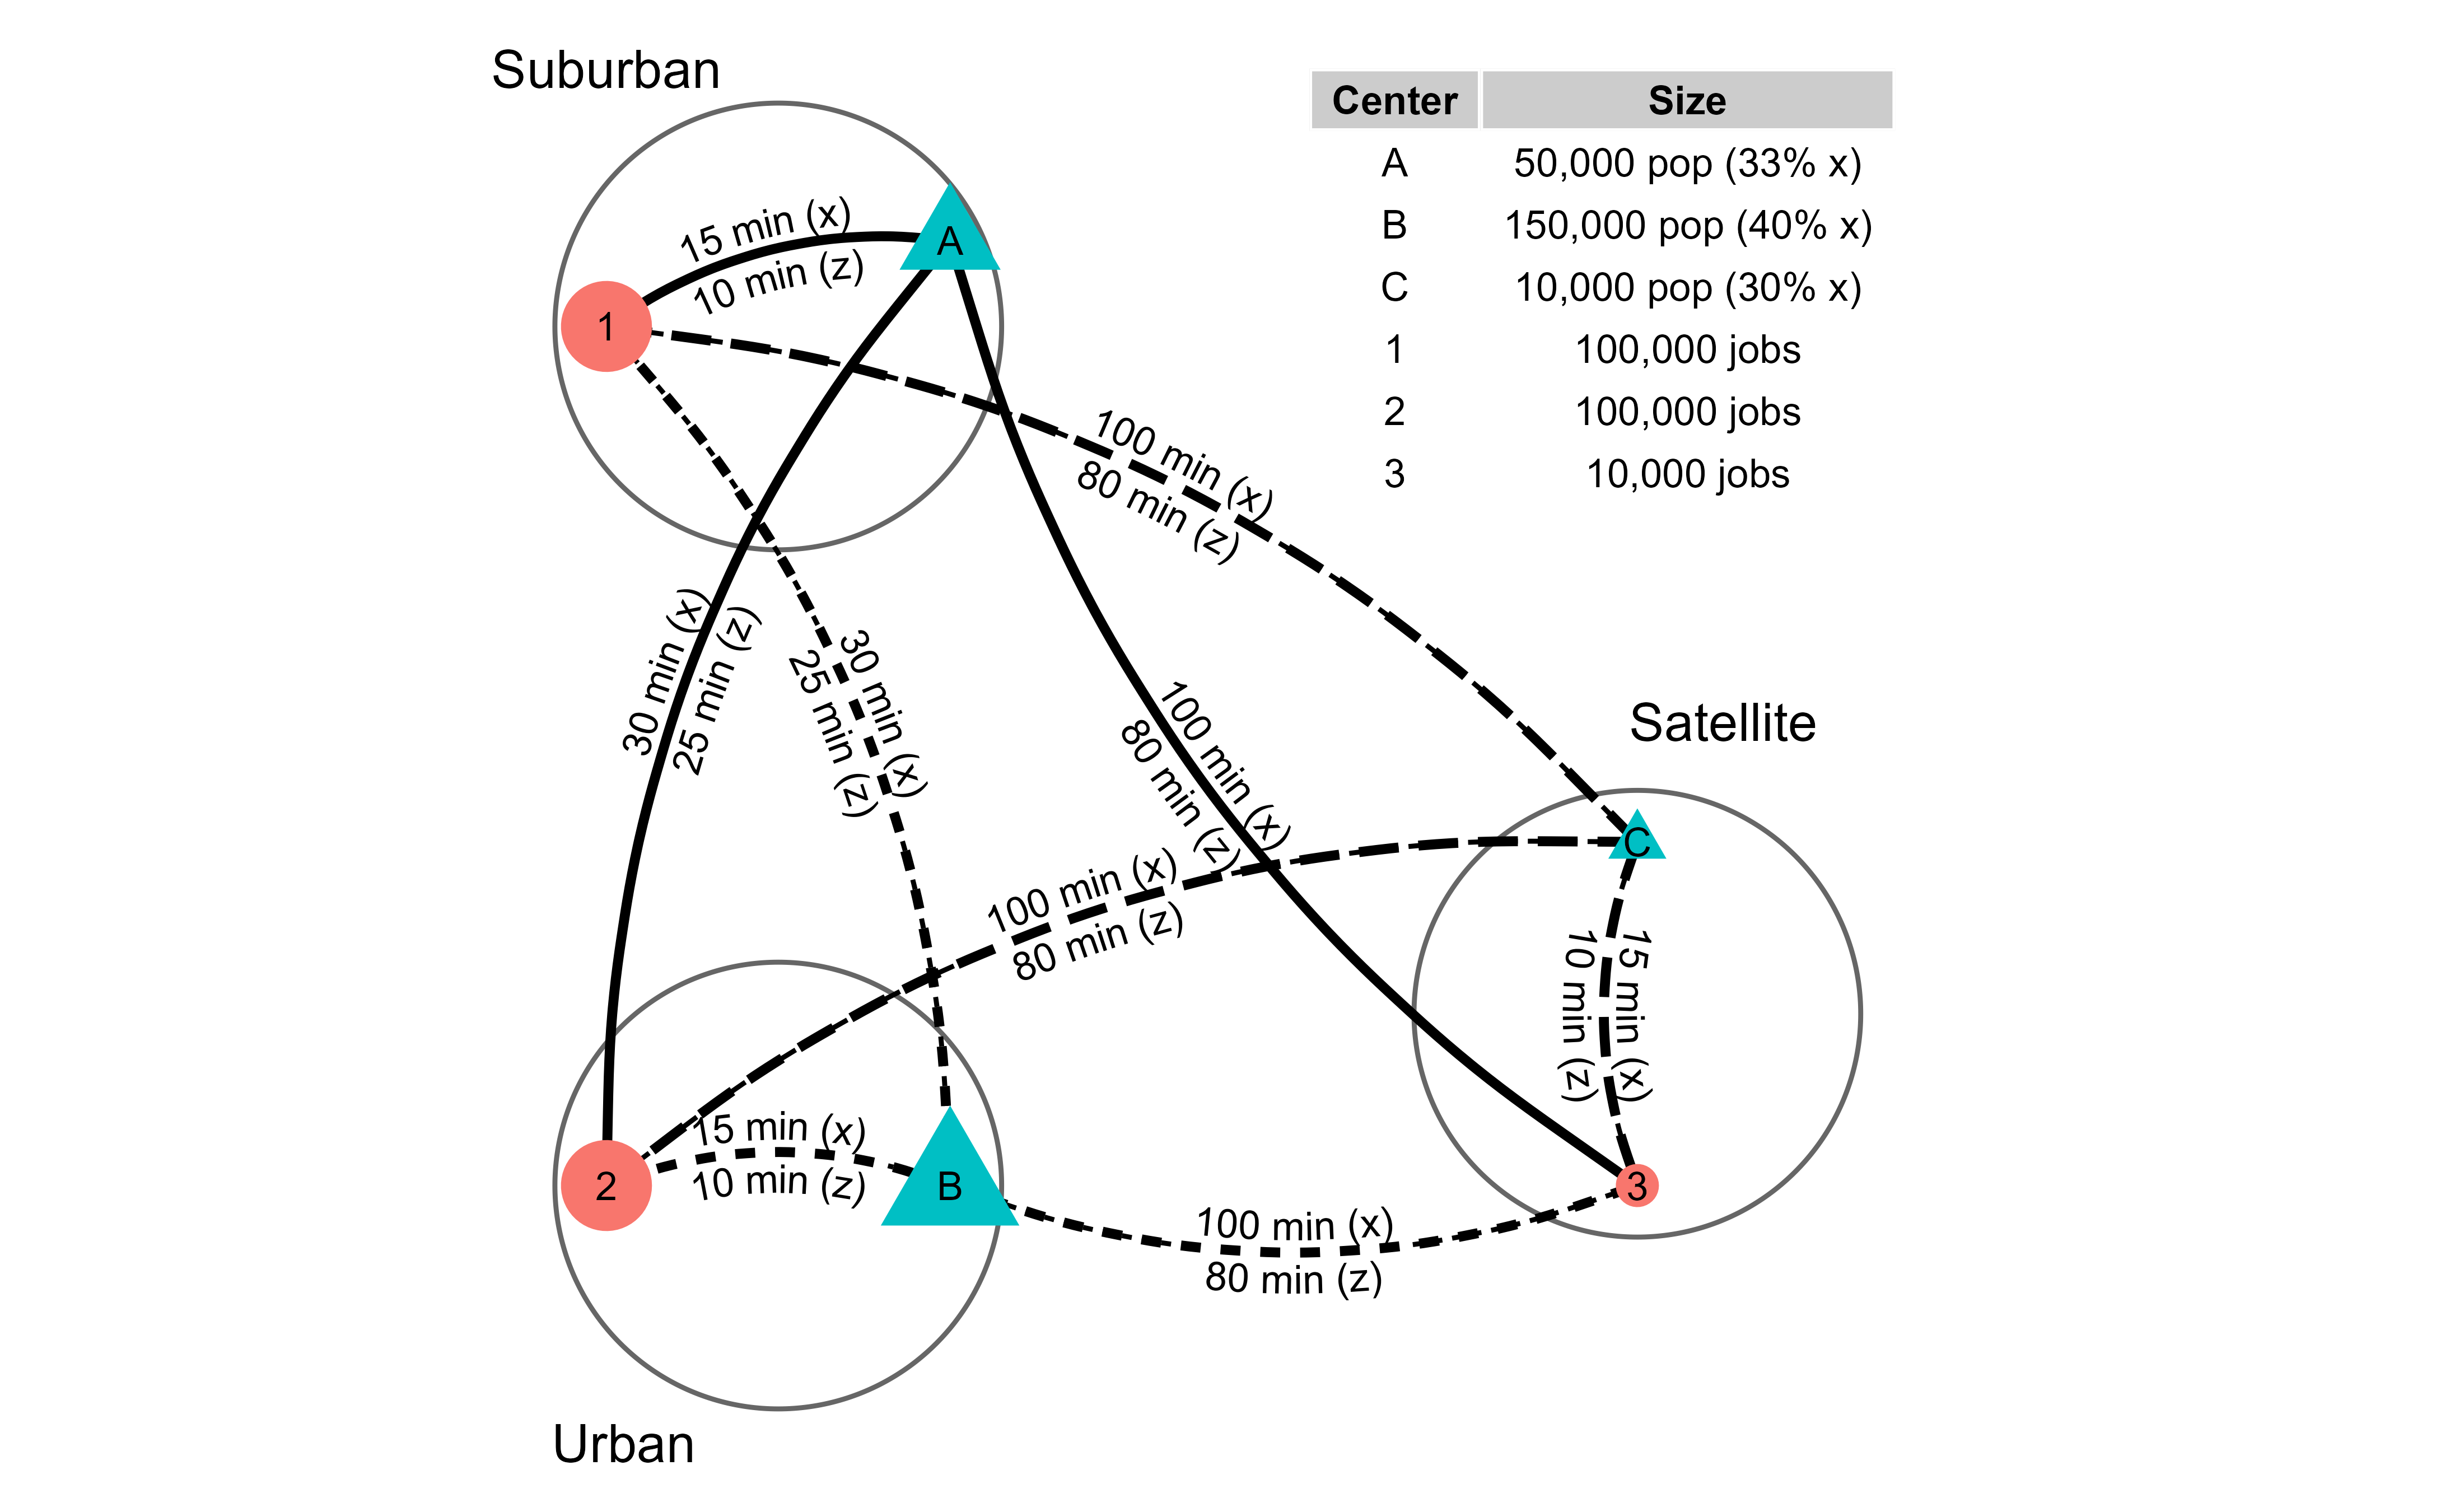
\includegraphics[width=1\linewidth]{images/Fig1} 

}

\caption{\label{fig:Fig1} Multimodal synthetic example: locations of employment centers (in orange), population centers (in blue), number of jobs and population, and travel times for two modes (slower mode x and faster mode z).}\label{fig:synthetic-example-plot}
\end{figure}

From the perspective of access to a \emph{finite} amount of
opportunities in the region (\(210,000\) jobs), the sub-population that
is most proximate to jobs, furthest from densely populated centers, and
is using the lowest travel-cost mode \(z\) can potentially access the
most job opportunities. This appears to be the sub-population at \(A\)
using \(z\). From the other perspective, sub-populations located in
opposite conditions (i.e., further away from jobs, close to dense
populations, and using \(x\)) are at a relative job opportunity access
\emph{disadvantage}. From the perspective of inequities, the competition
for opportunities between different mode-using populations matters as it
reflects how well the land-use and transport system serves (or doesn't
serve) them.

\global\setlength{\Oldarrayrulewidth}{\arrayrulewidth}

\global\setlength{\Oldtabcolsep}{\tabcolsep}

\setlength{\tabcolsep}{0pt}

\renewcommand*{\arraystretch}{1.5}



\providecommand{\ascline}[3]{\noalign{\global\arrayrulewidth #1}\arrayrulecolor[HTML]{#2}\cline{#3}}

\begin{longtable}[c]{|p{0.88in}|p{0.41in}|p{1.05in}|p{0.58in}|p{1.05in}|p{0.58in}|p{1.05in}}

\caption{Accessibility\ values\ at\ each\ origin\ per\ mode\ m\ at\ each\ origin\ i\ and\ aggregated\ between\ modes\ for\ each\ i\ for\ the\ synthetic\ example.}\\

\ascline{1.5pt}{666666}{1-7}

\multicolumn{1}{>{\raggedright}m{\dimexpr 0.88in+0\tabcolsep}}{\textcolor[HTML]{000000}{\fontsize{11}{11}\selectfont{i}}} & \multicolumn{1}{>{\raggedright}m{\dimexpr 0.41in+0\tabcolsep}}{\textcolor[HTML]{000000}{\fontsize{11}{11}\selectfont{m}}} & \multicolumn{1}{!{\color[HTML]{666666}\vrule width 1pt}>{\raggedleft}m{\dimexpr 1.05in+0\tabcolsep}}{\textcolor[HTML]{000000}{\fontsize{11}{11}\selectfont{S}}\textcolor[HTML]{000000}{\textsubscript{\fontsize{11}{11}\selectfont{i}}}\textcolor[HTML]{000000}{\textsuperscript{\fontsize{11}{11}\selectfont{m}}}} & \multicolumn{1}{>{\raggedleft}m{\dimexpr 0.58in+0\tabcolsep}}{\textcolor[HTML]{000000}{\fontsize{11}{11}\selectfont{a}}\textcolor[HTML]{000000}{\textsubscript{\fontsize{11}{11}\selectfont{i}}}\textcolor[HTML]{000000}{\textsuperscript{\fontsize{11}{11}\selectfont{m}}}} & \multicolumn{1}{>{\raggedleft}m{\dimexpr 1.05in+0\tabcolsep}}{\textcolor[HTML]{000000}{\fontsize{11}{11}\selectfont{V}}\textcolor[HTML]{000000}{\textsubscript{\fontsize{11}{11}\selectfont{i}}}\textcolor[HTML]{000000}{\textsuperscript{\fontsize{11}{11}\selectfont{m}}}} & \multicolumn{1}{!{\color[HTML]{666666}\vrule width 1pt}>{\raggedleft}m{\dimexpr 0.58in+0\tabcolsep}}{\textcolor[HTML]{000000}{\fontsize{11}{11}\selectfont{a}}\textcolor[HTML]{000000}{\textsubscript{\fontsize{11}{11}\selectfont{i}}}} & \multicolumn{1}{>{\raggedleft}m{\dimexpr 1.05in+0\tabcolsep}}{\textcolor[HTML]{000000}{\fontsize{11}{11}\selectfont{V}}\textcolor[HTML]{000000}{\textsubscript{\fontsize{11}{11}\selectfont{i}}}} \\

\ascline{1.5pt}{666666}{1-7}\endfirsthead \caption[]{Accessibility\ values\ at\ each\ origin\ per\ mode\ m\ at\ each\ origin\ i\ and\ aggregated\ between\ modes\ for\ each\ i\ for\ the\ synthetic\ example.}\\

\ascline{1.5pt}{666666}{1-7}

\multicolumn{1}{>{\raggedright}m{\dimexpr 0.88in+0\tabcolsep}}{\textcolor[HTML]{000000}{\fontsize{11}{11}\selectfont{i}}} & \multicolumn{1}{>{\raggedright}m{\dimexpr 0.41in+0\tabcolsep}}{\textcolor[HTML]{000000}{\fontsize{11}{11}\selectfont{m}}} & \multicolumn{1}{!{\color[HTML]{666666}\vrule width 1pt}>{\raggedleft}m{\dimexpr 1.05in+0\tabcolsep}}{\textcolor[HTML]{000000}{\fontsize{11}{11}\selectfont{S}}\textcolor[HTML]{000000}{\textsubscript{\fontsize{11}{11}\selectfont{i}}}\textcolor[HTML]{000000}{\textsuperscript{\fontsize{11}{11}\selectfont{m}}}} & \multicolumn{1}{>{\raggedleft}m{\dimexpr 0.58in+0\tabcolsep}}{\textcolor[HTML]{000000}{\fontsize{11}{11}\selectfont{a}}\textcolor[HTML]{000000}{\textsubscript{\fontsize{11}{11}\selectfont{i}}}\textcolor[HTML]{000000}{\textsuperscript{\fontsize{11}{11}\selectfont{m}}}} & \multicolumn{1}{>{\raggedleft}m{\dimexpr 1.05in+0\tabcolsep}}{\textcolor[HTML]{000000}{\fontsize{11}{11}\selectfont{V}}\textcolor[HTML]{000000}{\textsubscript{\fontsize{11}{11}\selectfont{i}}}\textcolor[HTML]{000000}{\textsuperscript{\fontsize{11}{11}\selectfont{m}}}} & \multicolumn{1}{!{\color[HTML]{666666}\vrule width 1pt}>{\raggedleft}m{\dimexpr 0.58in+0\tabcolsep}}{\textcolor[HTML]{000000}{\fontsize{11}{11}\selectfont{a}}\textcolor[HTML]{000000}{\textsubscript{\fontsize{11}{11}\selectfont{i}}}} & \multicolumn{1}{>{\raggedleft}m{\dimexpr 1.05in+0\tabcolsep}}{\textcolor[HTML]{000000}{\fontsize{11}{11}\selectfont{V}}\textcolor[HTML]{000000}{\textsubscript{\fontsize{11}{11}\selectfont{i}}}} \\

\ascline{1.5pt}{666666}{1-7}\endhead



\multicolumn{1}{>{\raggedright}m{\dimexpr 0.88in+0\tabcolsep}}{} & \multicolumn{1}{>{\raggedright}m{\dimexpr 0.41in+0\tabcolsep}}{\textcolor[HTML]{000000}{\fontsize{11}{11}\selectfont{x}}} & \multicolumn{1}{!{\color[HTML]{666666}\vrule width 1pt}>{\raggedleft}m{\dimexpr 1.05in+0\tabcolsep}}{\textcolor[HTML]{000000}{\fontsize{11}{11}\selectfont{27,292.18}}} & \multicolumn{1}{>{\raggedleft}m{\dimexpr 0.58in+0\tabcolsep}}{\textcolor[HTML]{000000}{\fontsize{11}{11}\selectfont{0.95}}} & \multicolumn{1}{>{\raggedleft}m{\dimexpr 1.05in+0\tabcolsep}}{\textcolor[HTML]{000000}{\fontsize{11}{11}\selectfont{18,959.86}}} & \multicolumn{1}{!{\color[HTML]{666666}\vrule width 1pt}>{\raggedleft}m{\dimexpr 0.58in+0\tabcolsep}}{} & \multicolumn{1}{>{\raggedleft}m{\dimexpr 1.05in+0\tabcolsep}}{} \\





\multicolumn{1}{>{\raggedright}m{\dimexpr 0.88in+0\tabcolsep}}{\multirow[c]{-2}{*}{\parbox{0.88in}{\raggedright \textcolor[HTML]{000000}{\fontsize{11}{11}\selectfont{A}}}}} & \multicolumn{1}{>{\raggedright}m{\dimexpr 0.41in+0\tabcolsep}}{\textcolor[HTML]{000000}{\fontsize{11}{11}\selectfont{z}}} & \multicolumn{1}{!{\color[HTML]{666666}\vrule width 1pt}>{\raggedleft}m{\dimexpr 1.05in+0\tabcolsep}}{\textcolor[HTML]{000000}{\fontsize{11}{11}\selectfont{44,999.80}}} & \multicolumn{1}{>{\raggedleft}m{\dimexpr 0.58in+0\tabcolsep}}{\textcolor[HTML]{000000}{\fontsize{11}{11}\selectfont{1.56}}} & \multicolumn{1}{>{\raggedleft}m{\dimexpr 1.05in+0\tabcolsep}}{\textcolor[HTML]{000000}{\fontsize{11}{11}\selectfont{46,913.04}}} & \multicolumn{1}{!{\color[HTML]{666666}\vrule width 1pt}>{\raggedleft}m{\dimexpr 0.58in+0\tabcolsep}}{\multirow[c]{-2}{*}{\parbox{0.58in}{\raggedleft \textcolor[HTML]{000000}{\fontsize{11}{11}\selectfont{1.32}}}}} & \multicolumn{1}{>{\raggedleft}m{\dimexpr 1.05in+0\tabcolsep}}{\multirow[c]{-2}{*}{\parbox{1.05in}{\raggedleft \textcolor[HTML]{000000}{\fontsize{11}{11}\selectfont{65,872.91}}}}} \\

\ascline{1pt}{666666}{1-7}



\multicolumn{1}{>{\raggedright}m{\dimexpr 0.88in+0\tabcolsep}}{} & \multicolumn{1}{>{\raggedright}m{\dimexpr 0.41in+0\tabcolsep}}{\textcolor[HTML]{000000}{\fontsize{11}{11}\selectfont{x}}} & \multicolumn{1}{!{\color[HTML]{666666}\vrule width 1pt}>{\raggedleft}m{\dimexpr 1.05in+0\tabcolsep}}{\textcolor[HTML]{000000}{\fontsize{11}{11}\selectfont{27,292.18}}} & \multicolumn{1}{>{\raggedleft}m{\dimexpr 0.58in+0\tabcolsep}}{\textcolor[HTML]{000000}{\fontsize{11}{11}\selectfont{0.62}}} & \multicolumn{1}{>{\raggedleft}m{\dimexpr 1.05in+0\tabcolsep}}{\textcolor[HTML]{000000}{\fontsize{11}{11}\selectfont{30,863.43}}} & \multicolumn{1}{!{\color[HTML]{666666}\vrule width 1pt}>{\raggedleft}m{\dimexpr 0.58in+0\tabcolsep}}{} & \multicolumn{1}{>{\raggedleft}m{\dimexpr 1.05in+0\tabcolsep}}{} \\





\multicolumn{1}{>{\raggedright}m{\dimexpr 0.88in+0\tabcolsep}}{\multirow[c]{-2}{*}{\parbox{0.88in}{\raggedright \textcolor[HTML]{000000}{\fontsize{11}{11}\selectfont{B}}}}} & \multicolumn{1}{>{\raggedright}m{\dimexpr 0.41in+0\tabcolsep}}{\textcolor[HTML]{000000}{\fontsize{11}{11}\selectfont{z}}} & \multicolumn{1}{!{\color[HTML]{666666}\vrule width 1pt}>{\raggedleft}m{\dimexpr 1.05in+0\tabcolsep}}{\textcolor[HTML]{000000}{\fontsize{11}{11}\selectfont{44,999.80}}} & \multicolumn{1}{>{\raggedleft}m{\dimexpr 0.58in+0\tabcolsep}}{\textcolor[HTML]{000000}{\fontsize{11}{11}\selectfont{1.03}}} & \multicolumn{1}{>{\raggedleft}m{\dimexpr 1.05in+0\tabcolsep}}{\textcolor[HTML]{000000}{\fontsize{11}{11}\selectfont{103,391.95}}} & \multicolumn{1}{!{\color[HTML]{666666}\vrule width 1pt}>{\raggedleft}m{\dimexpr 0.58in+0\tabcolsep}}{\multirow[c]{-2}{*}{\parbox{0.58in}{\raggedleft \textcolor[HTML]{000000}{\fontsize{11}{11}\selectfont{0.90}}}}} & \multicolumn{1}{>{\raggedleft}m{\dimexpr 1.05in+0\tabcolsep}}{\multirow[c]{-2}{*}{\parbox{1.05in}{\raggedleft \textcolor[HTML]{000000}{\fontsize{11}{11}\selectfont{134,255.38}}}}} \\

\ascline{1pt}{666666}{1-7}



\multicolumn{1}{>{\raggedright}m{\dimexpr 0.88in+0\tabcolsep}}{} & \multicolumn{1}{>{\raggedright}m{\dimexpr 0.41in+0\tabcolsep}}{\textcolor[HTML]{000000}{\fontsize{11}{11}\selectfont{x}}} & \multicolumn{1}{!{\color[HTML]{666666}\vrule width 1pt}>{\raggedleft}m{\dimexpr 1.05in+0\tabcolsep}}{\textcolor[HTML]{000000}{\fontsize{11}{11}\selectfont{2,240.38}}} & \multicolumn{1}{>{\raggedleft}m{\dimexpr 0.58in+0\tabcolsep}}{\textcolor[HTML]{000000}{\fontsize{11}{11}\selectfont{0.68}}} & \multicolumn{1}{>{\raggedleft}m{\dimexpr 1.05in+0\tabcolsep}}{\textcolor[HTML]{000000}{\fontsize{11}{11}\selectfont{2,034.49}}} & \multicolumn{1}{!{\color[HTML]{666666}\vrule width 1pt}>{\raggedleft}m{\dimexpr 0.58in+0\tabcolsep}}{} & \multicolumn{1}{>{\raggedleft}m{\dimexpr 1.05in+0\tabcolsep}}{} \\





\multicolumn{1}{>{\raggedright}m{\dimexpr 0.88in+0\tabcolsep}}{\multirow[c]{-2}{*}{\parbox{0.88in}{\raggedright \textcolor[HTML]{000000}{\fontsize{11}{11}\selectfont{C}}}}} & \multicolumn{1}{>{\raggedright}m{\dimexpr 0.41in+0\tabcolsep}}{\textcolor[HTML]{000000}{\fontsize{11}{11}\selectfont{z}}} & \multicolumn{1}{!{\color[HTML]{666666}\vrule width 1pt}>{\raggedleft}m{\dimexpr 1.05in+0\tabcolsep}}{\textcolor[HTML]{000000}{\fontsize{11}{11}\selectfont{3,745.89}}} & \multicolumn{1}{>{\raggedleft}m{\dimexpr 0.58in+0\tabcolsep}}{\textcolor[HTML]{000000}{\fontsize{11}{11}\selectfont{1.12}}} & \multicolumn{1}{>{\raggedleft}m{\dimexpr 1.05in+0\tabcolsep}}{\textcolor[HTML]{000000}{\fontsize{11}{11}\selectfont{7,837.22}}} & \multicolumn{1}{!{\color[HTML]{666666}\vrule width 1pt}>{\raggedleft}m{\dimexpr 0.58in+0\tabcolsep}}{\multirow[c]{-2}{*}{\parbox{0.58in}{\raggedleft \textcolor[HTML]{000000}{\fontsize{11}{11}\selectfont{0.99}}}}} & \multicolumn{1}{>{\raggedleft}m{\dimexpr 1.05in+0\tabcolsep}}{\multirow[c]{-2}{*}{\parbox{1.05in}{\raggedleft \textcolor[HTML]{000000}{\fontsize{11}{11}\selectfont{9,871.71}}}}} \\

\ascline{1pt}{666666}{1-7}



\multicolumn{1}{>{\raggedright}m{\dimexpr 0.88in+0\tabcolsep}}{\textcolor[HTML]{000000}{\fontsize{11}{11}\selectfont{TOTALS}}} & \multicolumn{1}{>{\raggedright}m{\dimexpr 0.41in+0\tabcolsep}}{\textcolor[HTML]{000000}{\fontsize{11}{11}\selectfont{}}} & \multicolumn{1}{!{\color[HTML]{666666}\vrule width 1pt}>{\raggedleft}m{\dimexpr 1.05in+0\tabcolsep}}{\textcolor[HTML]{000000}{\fontsize{11}{11}\selectfont{150,570.22}}} & \multicolumn{1}{>{\raggedleft}m{\dimexpr 0.58in+0\tabcolsep}}{\textcolor[HTML]{000000}{\fontsize{11}{11}\selectfont{N/A}}} & \multicolumn{1}{>{\raggedleft}m{\dimexpr 1.05in+0\tabcolsep}}{\textcolor[HTML]{000000}{\fontsize{11}{11}\selectfont{210,000.00}}} & \multicolumn{1}{!{\color[HTML]{666666}\vrule width 1pt}>{\raggedleft}m{\dimexpr 0.58in+0\tabcolsep}}{\textcolor[HTML]{000000}{\fontsize{11}{11}\selectfont{N/A}}} & \multicolumn{1}{>{\raggedleft}m{\dimexpr 1.05in+0\tabcolsep}}{\textcolor[HTML]{000000}{\fontsize{11}{11}\selectfont{210,000.00}}} \\

\ascline{1.5pt}{666666}{1-7}



\end{longtable}



\arrayrulecolor[HTML]{000000}

\global\setlength{\arrayrulewidth}{\Oldarrayrulewidth}

\global\setlength{\tabcolsep}{\Oldtabcolsep}

\renewcommand*{\arraystretch}{1}

The calculated \(S_i^m\), \(a_i^m\) and \(V_i^m\) accessibility values
for each \(i\) and \(m\) are shown in the middle three columns and are
aggregated for each \(i\) in the final two columns in Table 1 . We use a
negative exponential impedance function
\(f(c_{ij}) = \exp(-\beta\cdot c_{ij})\) with \(\beta=0.1\) for both
\(x\) and \(z\) modes for all accessibility measures calculations.

The Hansen-type measure \(S_i^m\) is presented for each origin and mode
in third column of Table 1 . For all \(i\), the \(z\)-using
sub-population has higher \(S_i^m\) values than the \(x\)-using
sub-populations. Additionally, \(S_i^m\) is equal for both mode-using
populations in \(A\) and \(B\). This is the case because \(S_i^m\) does
not consider \emph{competition}, it only relies on reflecting the count
of opportunities that may be interacted with as a product of
\(f^m(c_{ij}^m)\). Recall, populations in \(A\) and \(B\) have the same
travel impedance to employment centers \(1\), \(2\) and \(3\) (either
15, 30, or 100 minutes using \(x\) or 10, 25, or 80 minutes using
\(z\)). As such, these the calculated \(S_i^m\) values are the same for
both \(A\) and \(B\). Furthermore, the total sum of \(S_i^m\) in the
region is equal to 150,570.2. This value is difficult to interpret: it
represents the weighted sum of opportunities that may be interacted with
within the region based on travel impedance. It cannot be interpreted as
any sort of benchmark since the measure is \emph{non-constrained}. To
connect this example to literature, \(S_i^m\) is calculated in the work
of \citet{tahmasbiMultimodalAccessibilitybasedEquity2019}; they compare
differences in \(S_i^m\) values between modes in a relative and
comparative sense, but make no further interpretation of the \(S_i^m\)
values.

In the fourth and sixth column in Table 1 the Shen-type measure is
calculated: first for both origin and mode \(a_i^m\) as well as
aggregated by the weighted mean mode-population (
\(\sum_m \frac{P_i^m}{P_i}*a_i^m\) ) to represent a value for each
origin \(a_i\). Unlike \(S_i^m\), this measure considers
\emph{competition}. For instance, the \(x\)-using populations in \(A\)
and \(B\) centers do not have the same \(a_i^m\) values as the
\(z\)-using. In fact, \(A\) has the highest values \(a_i^m\) and \(a_i\)
values since this center has the smallest travel impedance to
opportunities (lower than at \(C\), \(A\) and \(B\) are equal) and has
one of these lowest proximity to a relatively high amount of population
(lower than at \(B\)).

However, the Shen-type measure is \emph{non-constrained}: the total sum
of \(a_i^m\) or \(a_i\) is practically meaningless since it represents a
sum of ratios. For instance, the \(z\)-using sub-population at \(A\) has
a value of 1.56 potential jobs per potential job-seeking population
compared to 0.95 for \(x\)-using sub-population. What is the
significance of these values? The difference between these modes is
equal to 0.62, but 0.62 of what? How many more job opportunities are
\(z\) users interacting with than \(x\) users? When \(a_i^m\) is
aggregated to \(a_i\) as shown in the sixth column, the values face
similar interpretability issues.

The Shen-type measure is implemented in the previously discussed work of
\citet{taoInvestigatingImpactsPublic2020a} to calculate modal \(a_i^m\)
values and the aggregated \(a_i\) is implemented in the work of
\citet{carpentieriMultimodalAccessibilityPrimary2020}. However, similar
to the Hansen-type measure, these works discuss relative and spatially
comparative differences in values, they do not make further
interpretation of the \(a_i^m\) or \(a_i\) themselves. This may be
because the Shen-type measure is \emph{non-constrained}, this is no
benchmark or global maximum to which comparisons can be drawn from.

By contrast, spatial availability \(V_i\) considers competition and is
constrained such that the total sum of values is equal to the total
number of opportunities in the region (i.e., \(210,000\) jobs). Seen in
fifth column of Table 1 , \(V_i^m\) for the same mode-using populations
in \(A\) and \(B\) are not the same (as this measure considers
competition). In fact, at \(A\), the \(z\)-using sub-population captures
27,953.18 more spatially available jobs (of the \(210,000\) jobs in the
region) than the sub-population using mode \(x\). The numerical
difference has a practical interpretation.

Furthermore, \(V_i^m\) values for an \(i\) can be aggregated across
\(m\) and compared across \(i\) ( \(V_i = \sum_m{\sum_i{V_i^m}}\) ) as a
result of the proportional allocation mechanism. This aggregation,
\(V_i\), is shown in the seventh column in Table 1 . Again looking at
center \(A\), \(A\) is allocated 65,872.91 spatially available
opportunities for both modes. 71\% of this spatial availability
allocated to \(A\) is assigned to the \(z\)-using population despite
representing 66\% of \(A\)'s population.

Spatial availability can be further aggregated to better interpret
competition between modes. Across the entire region, 137,500 people use
\(z\) (65\% of the region population). However, the \(z\)-using
population accounts for 75\% of the region's total spatial availability
- the rest is allocated to the \(x\)-using population (35\%of the total
population). Notably, the \(x\)-using population captures 10\% less
spatial availability to opportunities than its population proportion.
This understanding can lead us to ask normative questions such as, how
unequal should opportunity access for the two mode-using populations be?
Can the lower-travel-cost populations spare some spatial availability if
a policy of modal-restriction (like a LEZ) was introduced?

Alternatively, inequities in spatial availability between mode-using
populations can be explored through proportional benchmarks. A spatial
availability per capita \(v_i^m\) as presented in Equation
(\ref{eq:SA-per-capita}):

\begin{equation}
\label{eq:SA-per-capita}
v_{i}^m = \frac{V_{i}^m}{P_{i}^m}
\end{equation}

The \(v_i^m\) values for \(A\), \(B\), and \(C\) for the \(x\)-using
sub-populations are 0.95, 0.62 and 0.68 spatially available jobs per
capita, respectively. The \(v_i^m\) for the \(z\)-using sub-populations
are much higher, with values of: 1.56, 1.03 and 1.12 respectively. The
\(x\)-using population, especially at \(B\) and \(C\), are directly
impacted by the jobs that are spatially available to the \(z\)-using
population \emph{in addition to} the mass effect (occurring at \(B\),
high population density) and high travel impedance (occurring at the
Satellite \(C\)).

If, lets say, the planning goal is to have one spatially available job
per mode-using population, a policy intervention can be put in place, to
reduce the \(v_i^z\) values and increase \(v_i^x\) values. This
demonstration is to show how simply the \(V_i^m\) framework can be
manipulated quantify the competitive (dis)advantage in a multimodal
application. In what follows, we further explore competition between
multiple modes through an empirical example.

\hypertarget{empirical-example-madrid-lez}{%
\section{Empirical example: Madrid
LEZ}\label{empirical-example-madrid-lez}}

\hypertarget{multimodal-data-and-methods}{%
\subsection{Multimodal data and
methods}\label{multimodal-data-and-methods}}

Low emission zones (LEZ) have been implemented as a climate change
policy intervention to reduce GHG emissions, improve air quality, and
support sustainable mobility in many countries. Though rules vary, LEZ
aim to deter/reduce traffic in designated zones under threat of penalty
(e.g., fines, seizure of vehicle). From the perspective of restriction
for passenger transport, LEZ are a policy of \emph{geographic
discrimination}. LEZ actively change how people access opportunities by
making the travel impedance more costly for car-mode users. If seeing
opportunities as finite, this discrimination allows populations to
access opportunities by other modes more readily than before. In this
way, LEZ change the multimodal competitive accessibility landscape of a
city.

Spain is one of a few countries with active LEZ and plans to expand
their implementation as specified in their climate-change-related plans:
\emph{Plan Nacional Integrado de Energía y Clima 2021-2030}
\citep{espanaPlanNacionalIntegrado2020} and \emph{Plan Nacional de
Control de la Contaminación Atmosférica}
\citep{espanaResolucion10Enero2020}. Specifically, the national Spanish
law 7/2021 ( \emph{Ley de Cambio Climático y Transición Energética})
will require all municipalities to implement LEZ by 2023 if they meet at
least one of the following requirements: (i) municipalities
\textgreater50,000 inhab.; (ii) islands; and (iii) municipalities
\textgreater{} 20,000 inhab. when air quality exceeds limits specified
in \emph{RD 102/2011 de Mejora de Calidad del Aire}
\citep{barcelonaGUIATECNICAPARA2021}.

In 2017, a LEZ was implemented in the Spanish capital city of Madrid
following the goals set out in the national agenda . In geographic
scope, the 2017 boundaries of the LEZ were relatively small (covering
4.72 km\^{}\{2\}) and within the center (i.e., LEZ Centro). These
boundaries were expanded in 2023 to inside of the M-30, a highway in
proximity to the city center (i.e., LEZ M-30) and the city has plans to
further spatially expand the LEZ. Within the 2017 LEZ Centro
implementation, all cars, motorcycles and freight with environmental
label A or B (higher polluting classification, associated with older
make and model of fossil fuel internal combustion engine vehicles), are
banned from driving into the area (threat of fine) unless they are used
by residents or meet other exemptions. This restriction impacted
approximately half of all car trips that were typically made into the
LEZ Centro \citep{tarrinoortizAnalyzingImpactLow2022}.

In this section, we use \(V_i^m\) to quantify the competition for
spatially available opportunities between modes after the LEZ Centro
implementation. Particularly, we demonstrate how \(V_i^m\) can be used
to spectate on how the restriction of car mobility in areas
around/within the LEZ Centro allowed the other, more sustainable but
often with higher travel impedance modes, to become more competitive.

\begin{figure}

{\centering 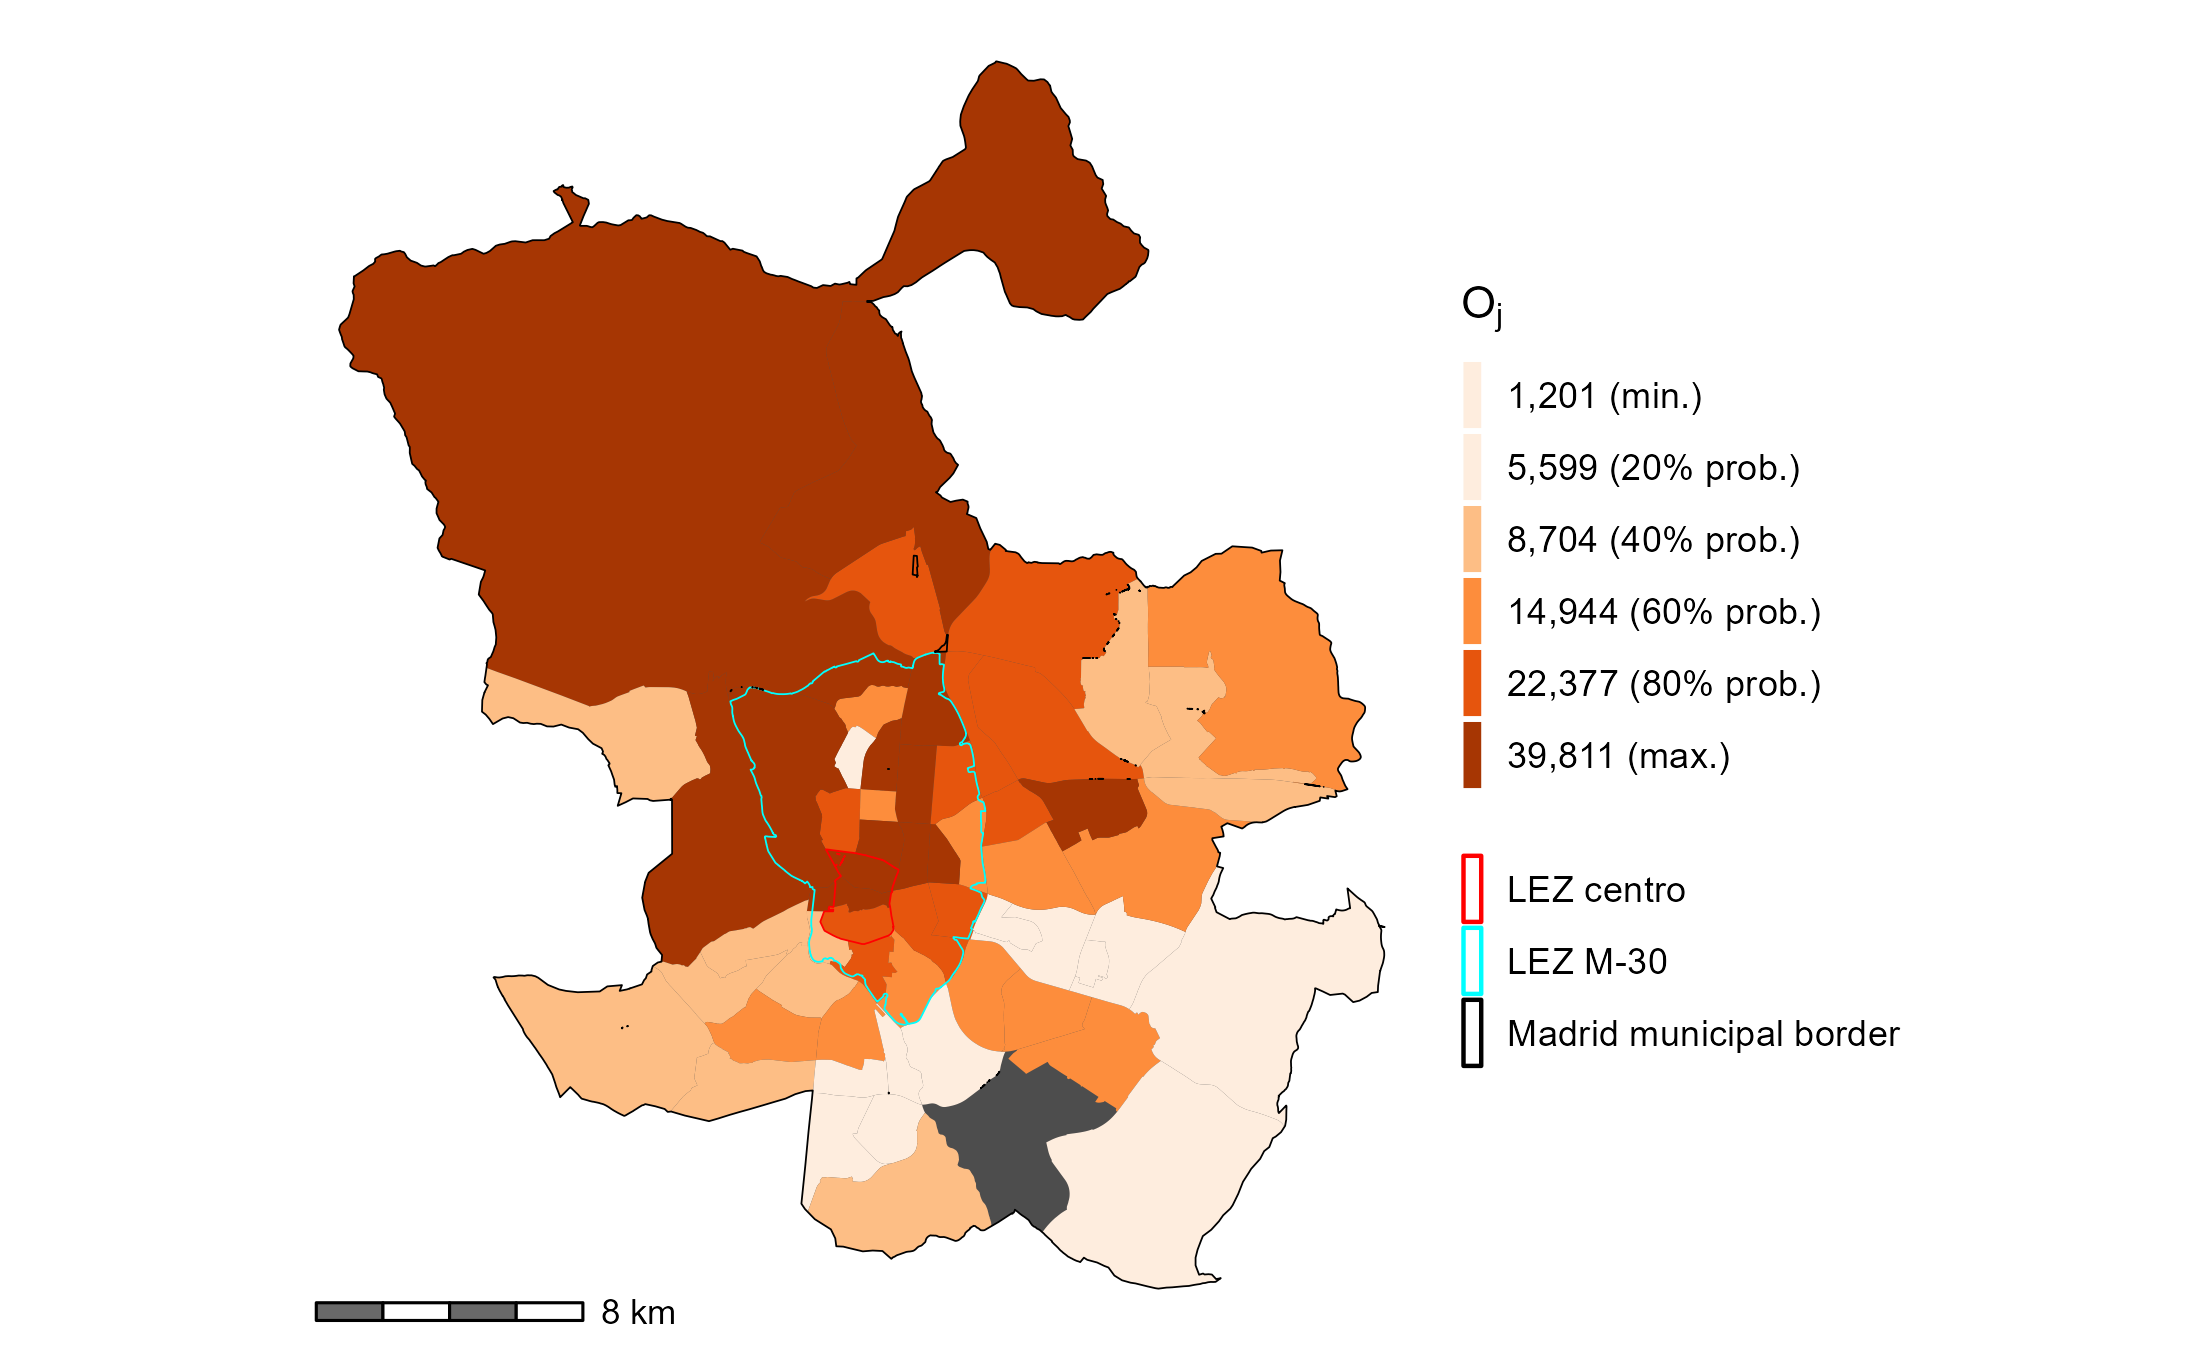
\includegraphics[width=1\linewidth]{images/i_jobs_zn208_plot} 

}

\caption{\label{fig:Fig2} Jobs $O_j$ taken by people living and working in Madrid as reported by the 2018 travel survey.}\label{fig:jobs-plot}
\end{figure}

\begin{figure}

{\centering 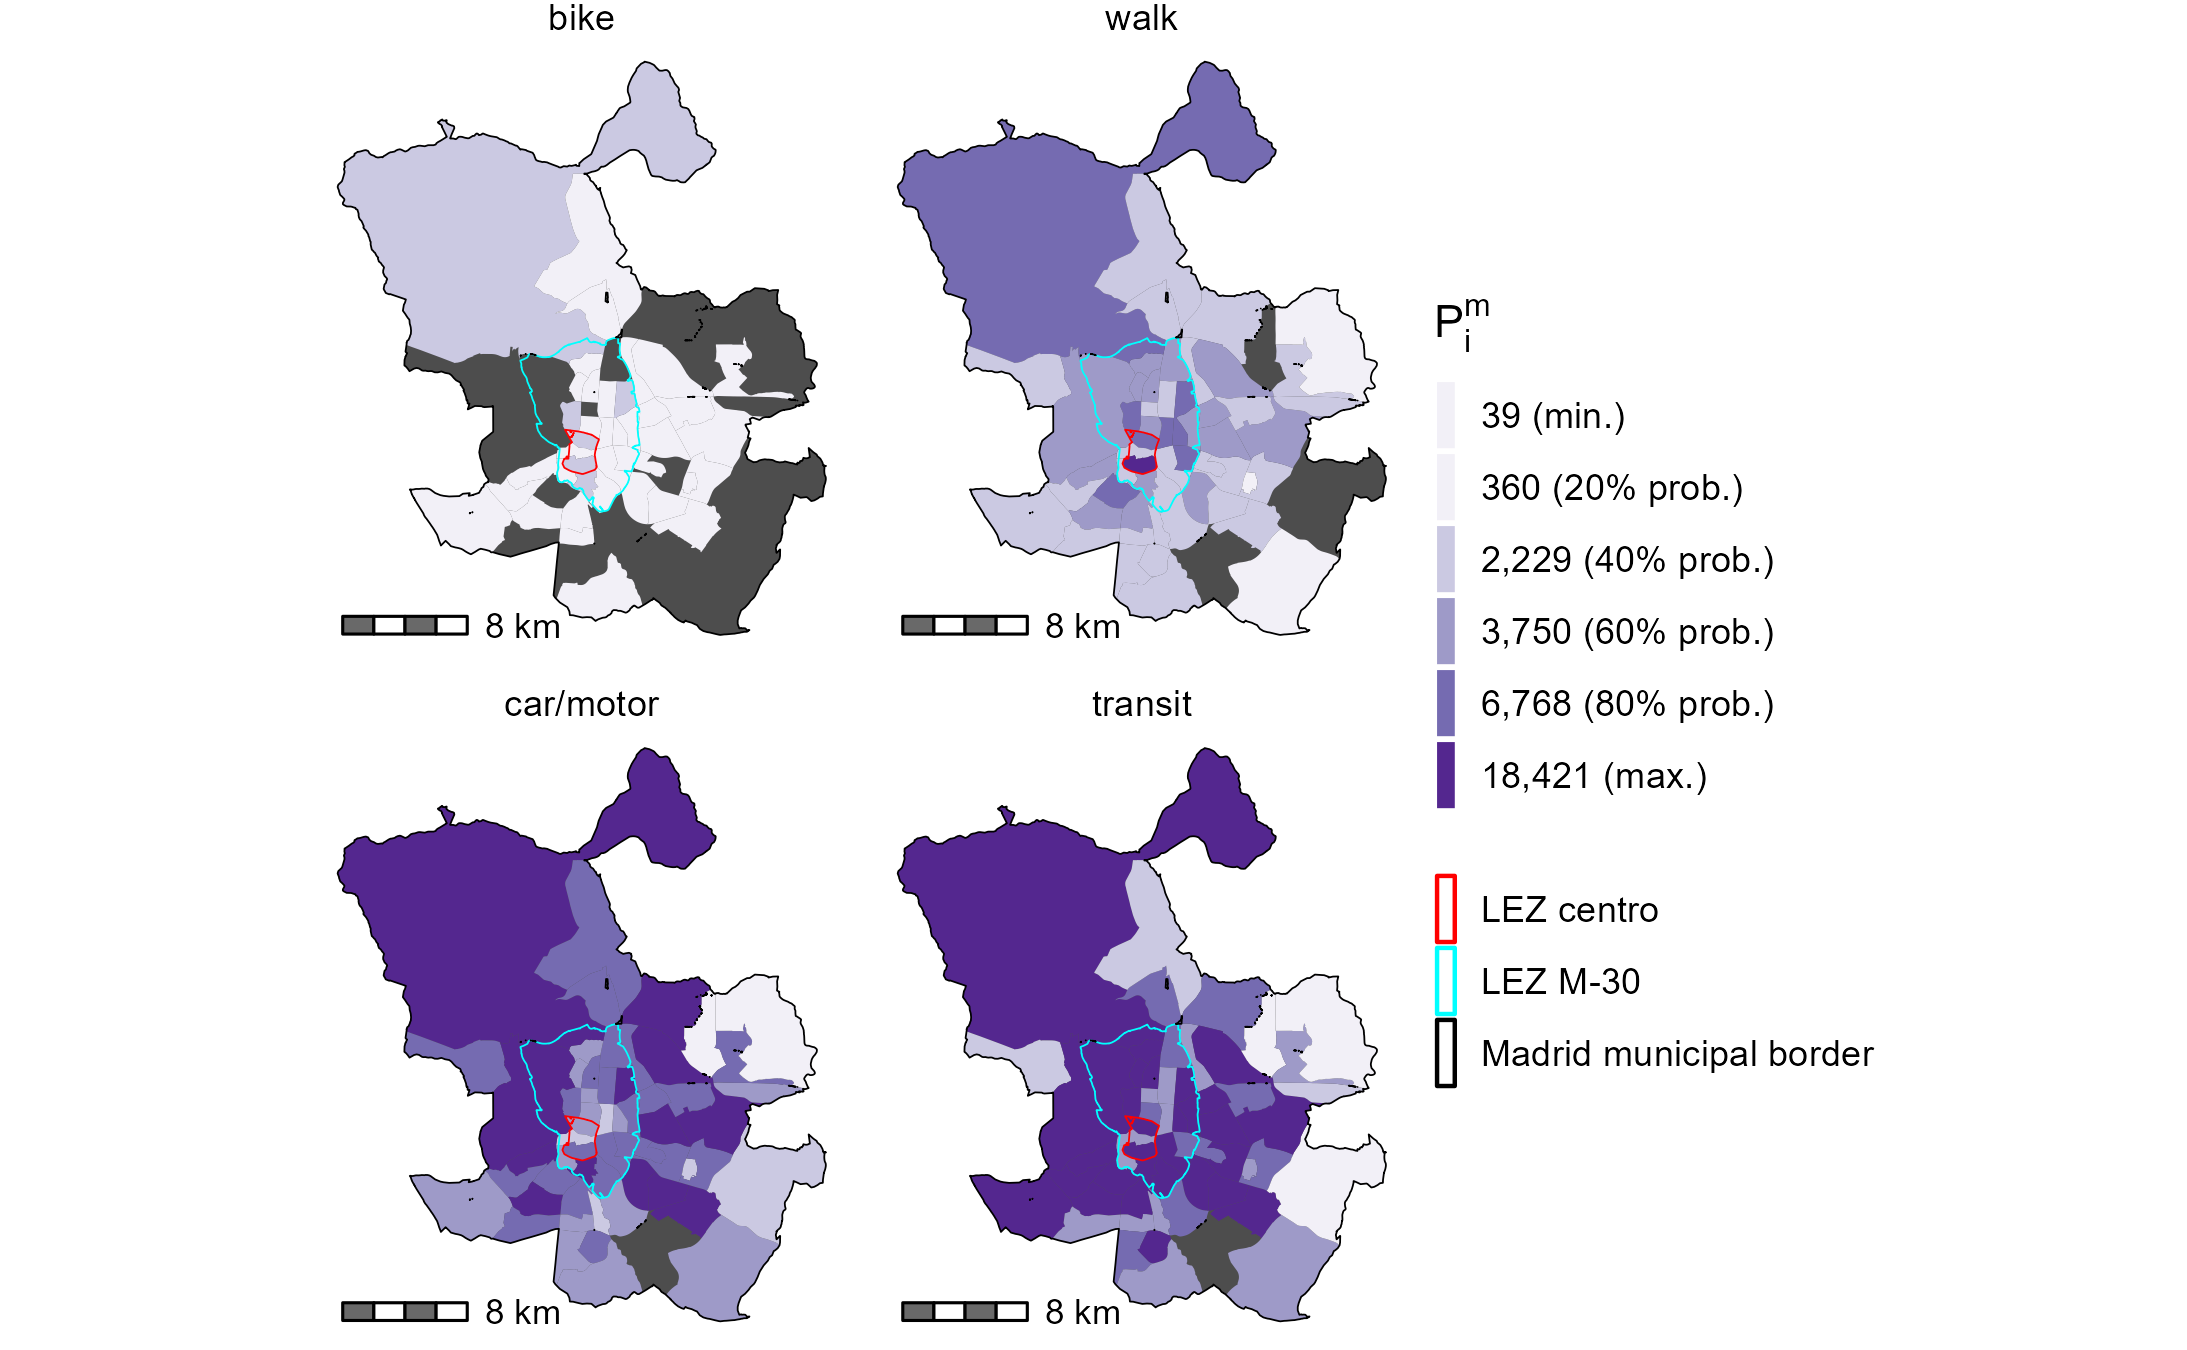
\includegraphics[width=1\linewidth]{images/im_populations_zn208_plot} 

}

\caption{\label{fig:Fig3} Population living and working in Madrid, by four summarized modal categories, $P^m_i$ as reported by the 2018 travel survey.}\label{fig:pop-plot}
\end{figure}

The 2018 Community of Madrid travel survey
(\citet{comunidaddemadridResultadosEDM20182020}) is the source of data
for this empirical example: it is a representative survey that reflects
a snap-shot of the travel patterns for one typical day of the working
week (e.g., n=222,744 trips with representative population elevation
factors). In this paper, a sample of the travel survey is used, namely
the residential home origin to work destination trips of all modes and
those that originate and end in the city of Madrid. These totals are
displayed in Figure \ref{fig:Fig2} and Figure \ref{fig:Fig3}. Both
figures are displayed at the level of traffic analysis zones (\(i\) and
\(j\)) that correspond to the survey. The red boundary represents the
LEZ Centro in effect in 2017 and thus those travel patterns of
car-restriction reflected in the survey. The cyan boundary represents
the LEZ that will be within the boundaries of the M-30 highway in 2023
and is present in the plots as a spatial reference for areas in
proximity to the LEZ Centro.

The total sum of jobs \(O_j\) that are held are shown in Figure
\ref{fig:Fig2} and the populations that go to a work destination by four
modal categories \(P^m_i\), is reflected in Figure \ref{fig:Fig3}. The
modal categories represented in Figure \ref{fig:Fig3} are summarized for
the following trip mode types:

\begin{itemize}
\tightlist
\item
  Car/motor: all cars and operating modes (e.g., cab, private driver,
  company, rental care, main driver, passenger, etc.) and all public,
  private or company motorcycle/mopeds.
\item
  Transit: all bus, trams, and trains
\item
  Bike: all bicycle trips (e.g., private, public, or company bike trips)
  and ``other'' types of micromobility options
\item
  Walk: walking or by foot
\end{itemize}

From Figure \ref{fig:Fig2}, it can be seen that the largest
concentration of jobs are within, near, and to the north of the LEZ
Centro. The population that is accessing those jobs by mode (Figure
\ref{fig:Fig3}), appear spatially distinct. Car and transit trips
represent 37\% and 47\% of the modal share respectively. The population
that travels using transit is more spatially distributed than those
using cars - particularly near and within LEZ Centro. This distribution
could be a result of a variety of factors including: transit coverage
and service within with city, effective car infrastructure outside of
the M-30, and/or the impact of the Central LEZ itself.

From Figure \ref{fig:Fig2}, it can also be seen that biking and walking
trips are less common than motorized trips at 1\% and 15\% respectively.
The distribution of walking and biking trips appear to be similar to
that of transit trips.

The travel time for each trip is provided within the survey. These
travel times, per modal category, are used to calibrate mode-specific
travel impedance functions \(f^m(c_{ij}^m)\). To illustrate the modal
differences in travel lengths, summary descriptive per mode are
detailed:

\begin{itemize}
\tightlist
\item
  Car/motor: 36 min (min:0 min., Q2: 15 min., Q3: 55 min., max: 120
  min.)
\item
  Transit: 55 min. (min:1 min., Q2: 30 min., Q3: 80 min., max: 120 min.)
\item
  Bike: 34 min. (min:5 min., Q2: 15 min., Q3: 40 min., max: 115 min.)
\item
  Walk: 27 min. (min:1 min., Q2: 10 min., Q3: 45 min., max: 119 min.)
\end{itemize}

To calculate \(f^m(c_{ij}^m)\) from the survey travel times, a concept
known as the trip length distribution (TLD) was used. A TLD represents
the proportion of trips that are taken at a specific travel cost such as
travel time (i.e., probability density distribution of trips taken by
travel cost). This distribution is then used to derive impedance
functions \citep[e.g., done in the accessibility works
of][\citet{horbachov_theoretical_2018}, and
\citet{batista_estimation_2019} for example]{lopez_2017_spatial}.
Maximum likelihood estimation and the Nelder-Mead method for direct
optimization available within the R \{fitdistrplus\} package
\citep{fitdistrplus_2015} is used to fit the impedance functions. As
shown as shown in Figure \ref{fig:Fig4}, based on goodness-of-fit
criteria and associated diagnostics, the gamma and log-normal
probability density function (line curves) are selected as best fitting
curves for the motorized and non-motorized modes respectively. The
selection of functional form aligns with examples used in the literature
(e.g., \citet{reggianiAccessibilityImpedanceForms2011}). Overall, the
plots in Figure \ref{fig:Fig4} display the probability of travel given a
trip travel time, based on trip flows from the survey. These
`probability of travel' at each travel time for each mode are realized
observations reflect the land-use, the transport system, and the
population travel behaviour in Madrid.

\begin{figure}

{\centering 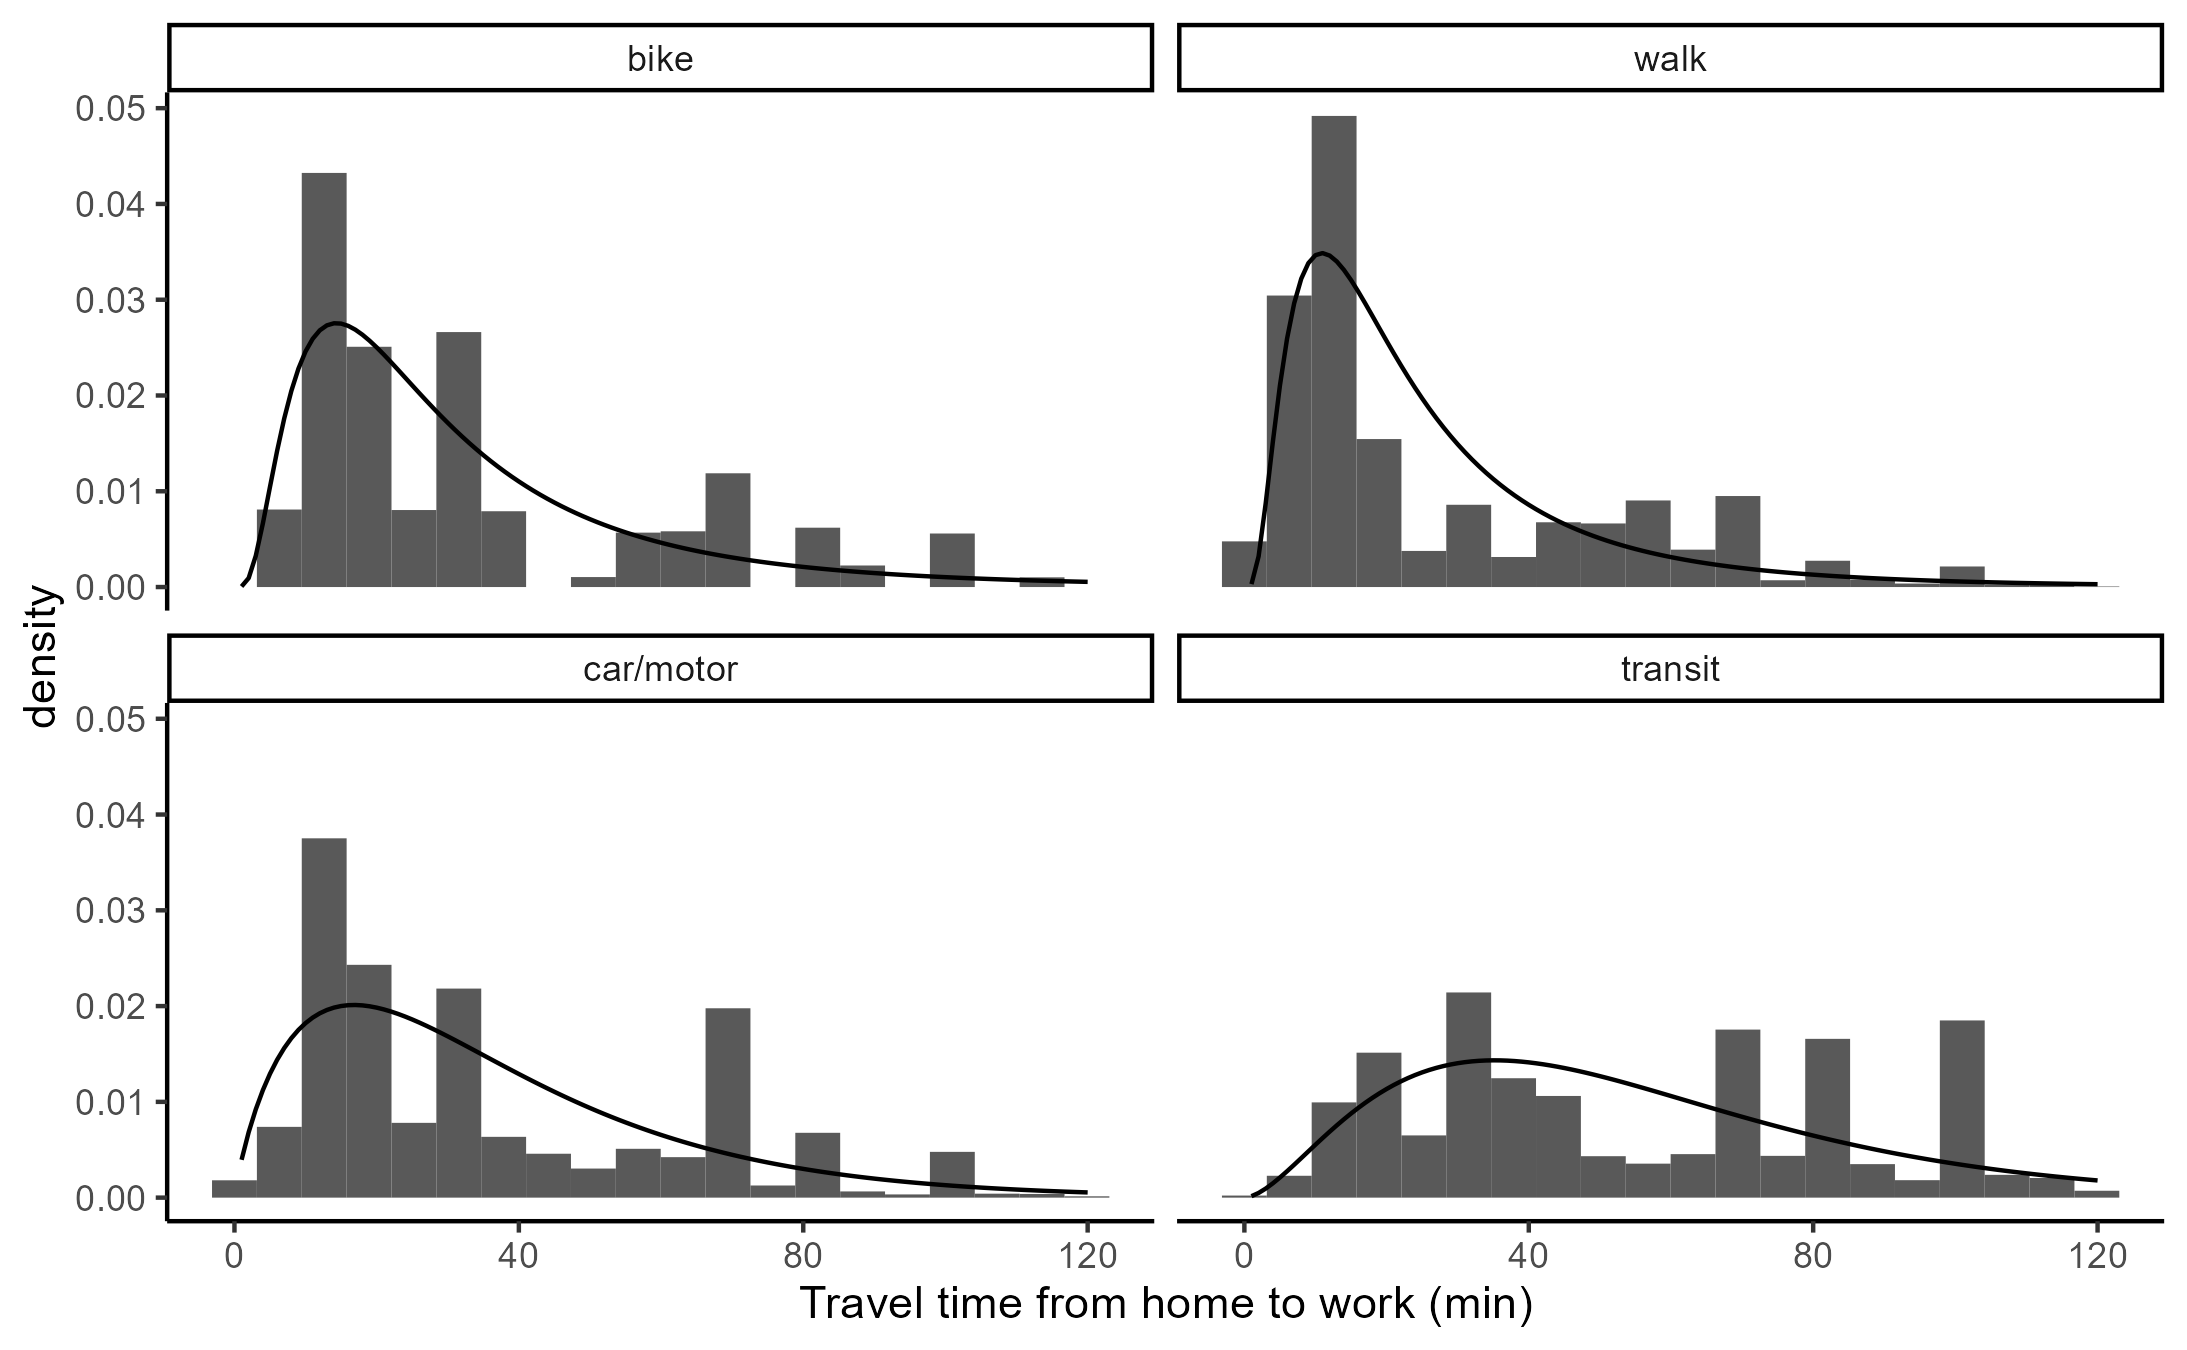
\includegraphics[width=1\linewidth]{images/tlds_curves_m_plot} 

}

\caption{\label{fig:Fig4} Fitted impedance function curve (line) against empirical TLD (bars) corresponding to the home-to-work origin-destination flows from the Madrid 2018 travel survey.}\label{fig:tlds-curves-m-plot}
\end{figure}

\hypertarget{results}{%
\subsection{Results}\label{results}}

Using the data inputs outlined, \(V_i^m\), the spatial availability of
jobs, is calculated for each of the four modal categories \(m\) at the
level of traffic analysis zones \(i\) in Madrid and demonstrated in this
sub-section.

\begin{figure}

{\centering 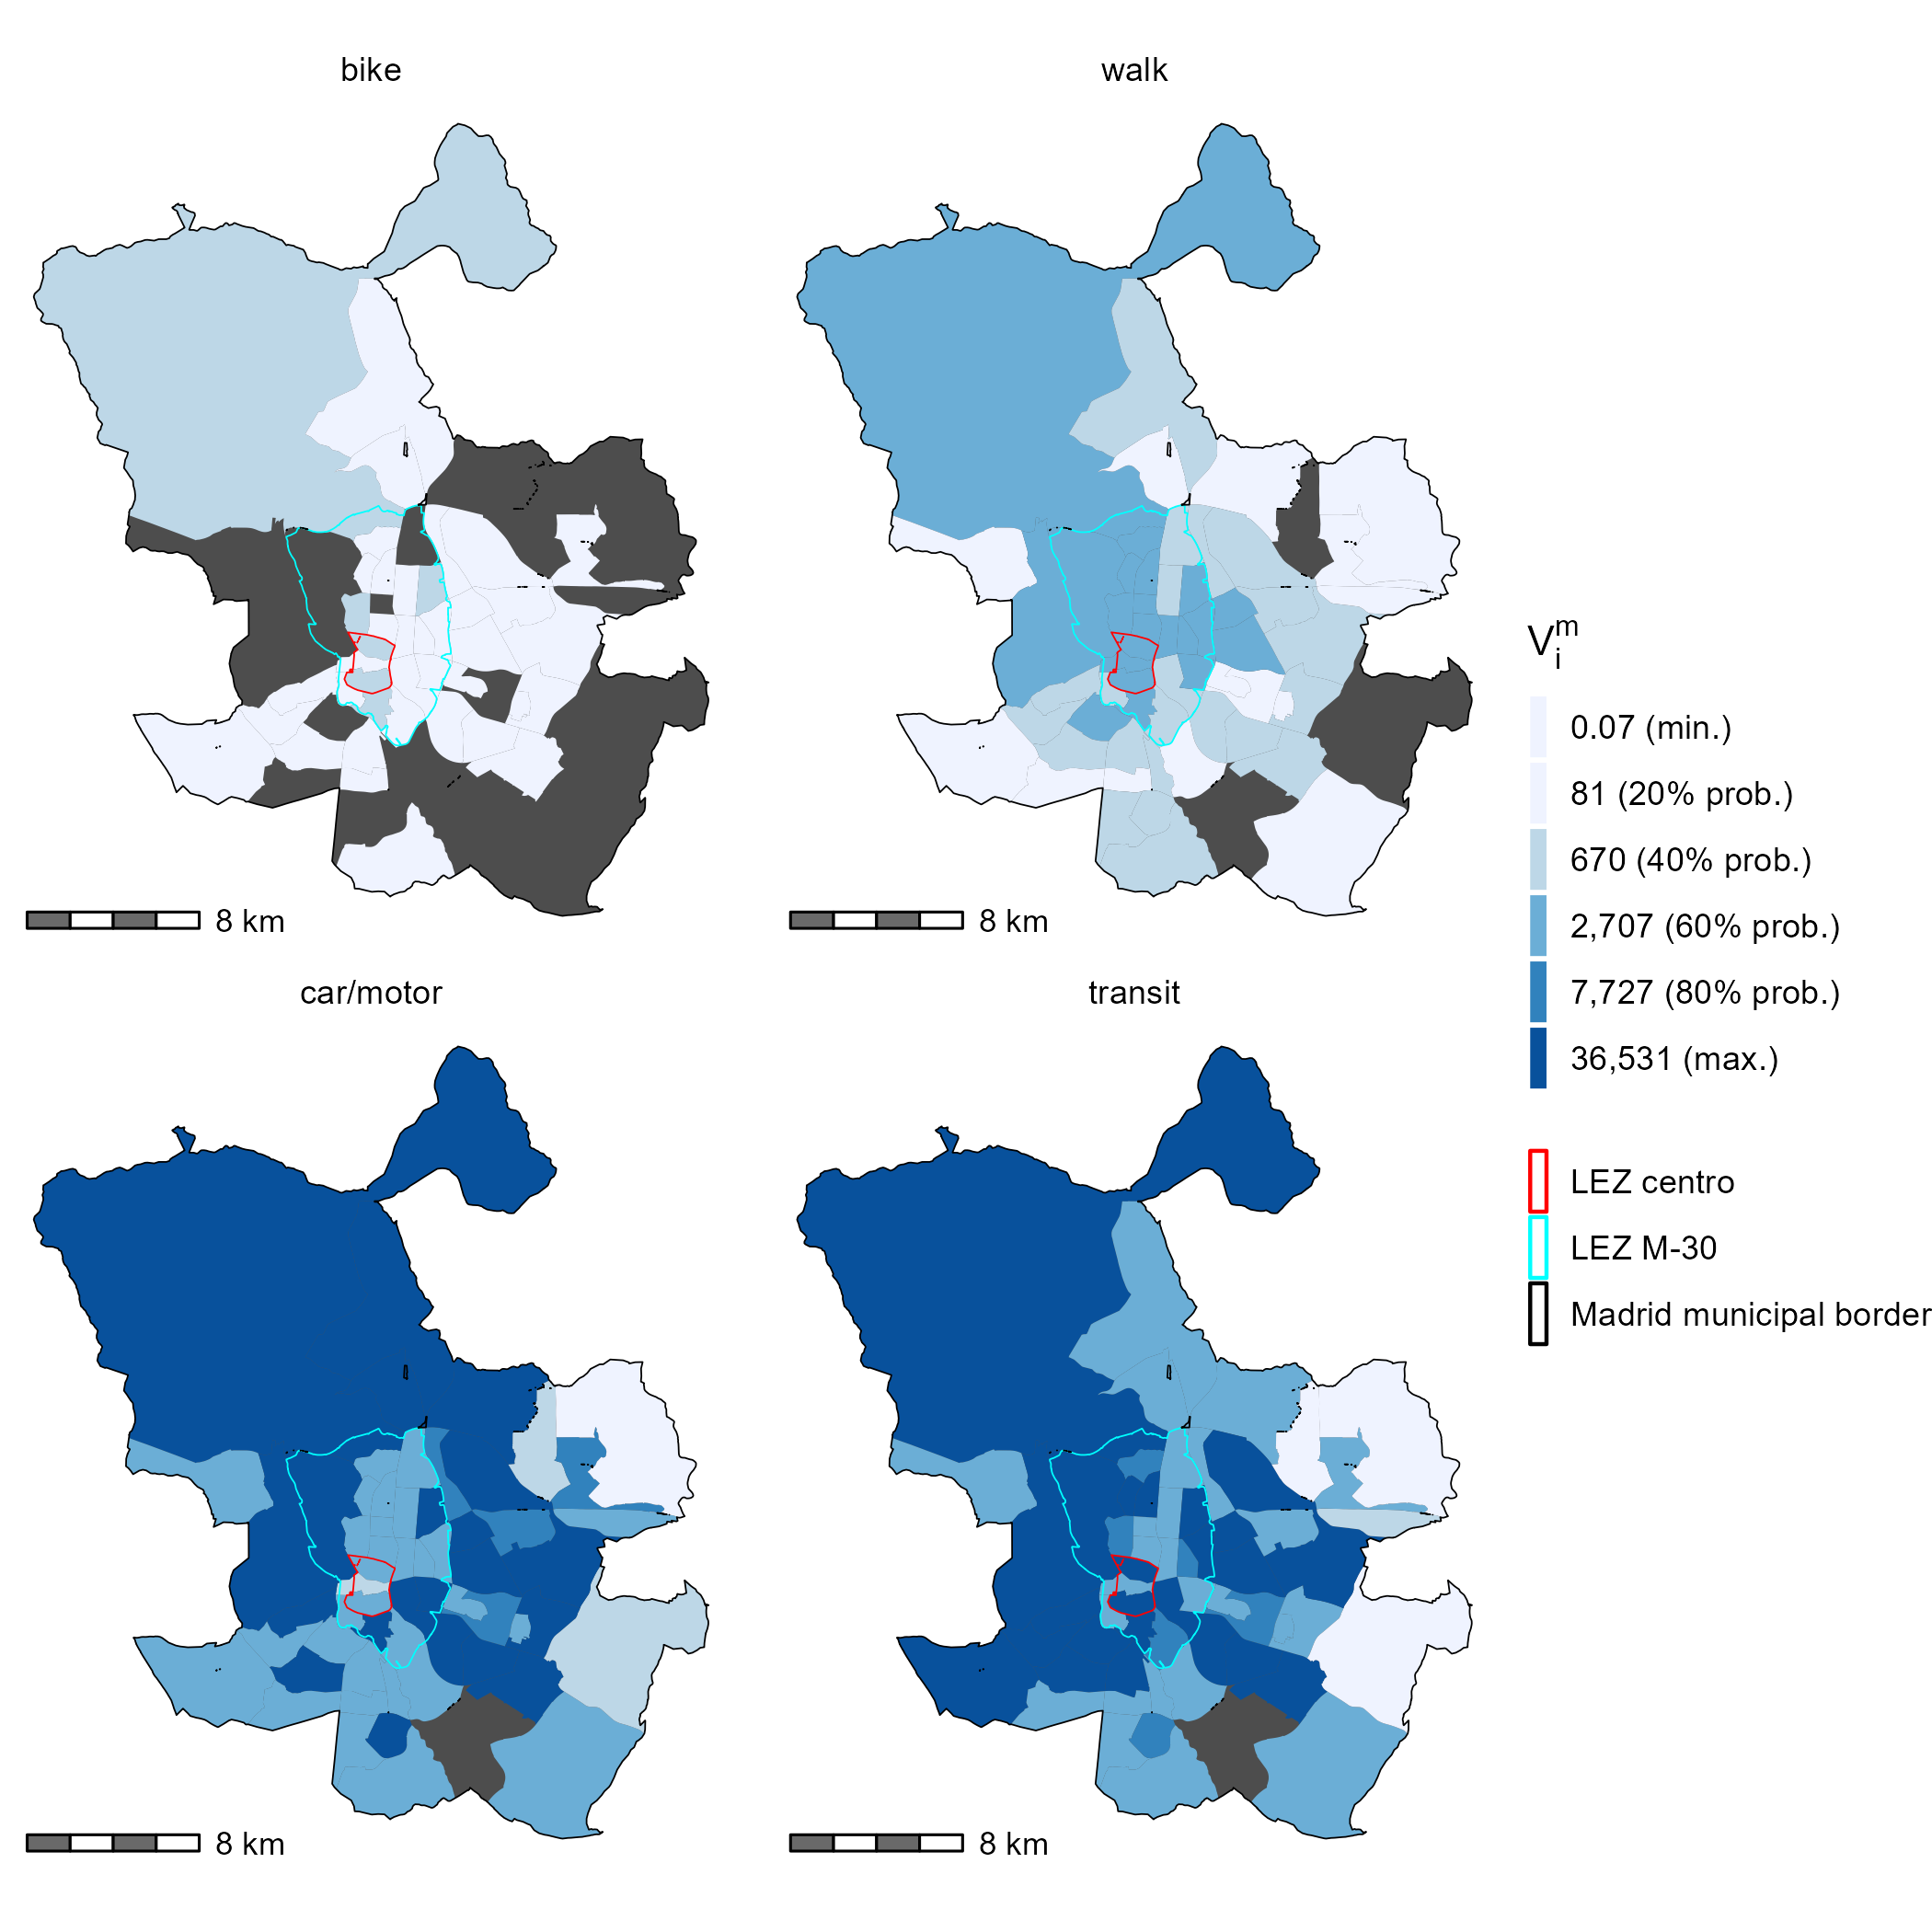
\includegraphics[width=1\linewidth]{images/SA_im_V_zn208_plot} 

}

\caption{\label{fig:Fig5} Spatial availability of job opportunities per origin and mode $V_i^m$ in Madrid. Calculated using the home-to-work origin-destination flows from the 2018 travel survey. }\label{fig:SA-m-plot}
\end{figure}

Figure \ref{fig:Fig5} displays \(V_i^m\) for the four modal categories
in 2018. \(V_i^m\) values represent a proportion of the total number of
the 847,574 jobs in the region; put another way, \(V_i^m\) is how many
jobs are \emph{spatially available} to the population located at the
\(i\) based on the travel impedance of the mode (relative to the travel
impedance of all modes) and the mode-using population size at the \(i\)
(relative to the population size of all modes and \(i\)). Note the
differences in the magnitudes of \(V_i^m\) between modes. The majority
of \(V_i^m\) is allocated to car- and transit- using populations. This
is to be expected, as commuting using motorized modes represents 84\% of
the population (37\% (car/motor) and 47\% (transit) in 2018). However,
these modal options capture 95\% of the total spatial availability in
Madrid. In particular, the car/motor using population is allocated
disproportionately more \(V_i^m\) than its modal population (37\% of the
population vs.~48\% of the \(V_i^m\)) compare to the transit using
population and its relatively proportional \(V_i^m\) value (15\% of the
population vs.~47\% \(V_i^m\)).

How does the \(V_i^m\) advantage allocated to car-using population
arise? From the perspective of finite opportunities, \(V_i^m\) is
allocated to car-using populations from less competitive modal
populations. How competitive one mode is compared to other modes varies
spatially, but overall car-using populations capture more opportunities
per car-using population than other modal populations. Namely, though
walking and cycling populations represent 14.74\% and 1.16\%
respectively, \(V_i^m={walk}\) and \(V_i^m={bike}\) is 4.43\% and 0.23\%
in the region respectively. These modes are less competitive, especially
compared to the car/motor mode, as a result of: 1) their lower travel
impedance values at longer travel times (see Figure \ref{fig:Fig4} at
travel times beyond \textasciitilde30 minutes), 2) their low population
values values overall, and 3) higher populations present in origins with
high motorized mode commuting. These factors all contribute to the the
car/motor mode being most advantaged in capturing spatially available
job opportunities overall.

\begin{figure}

{\centering 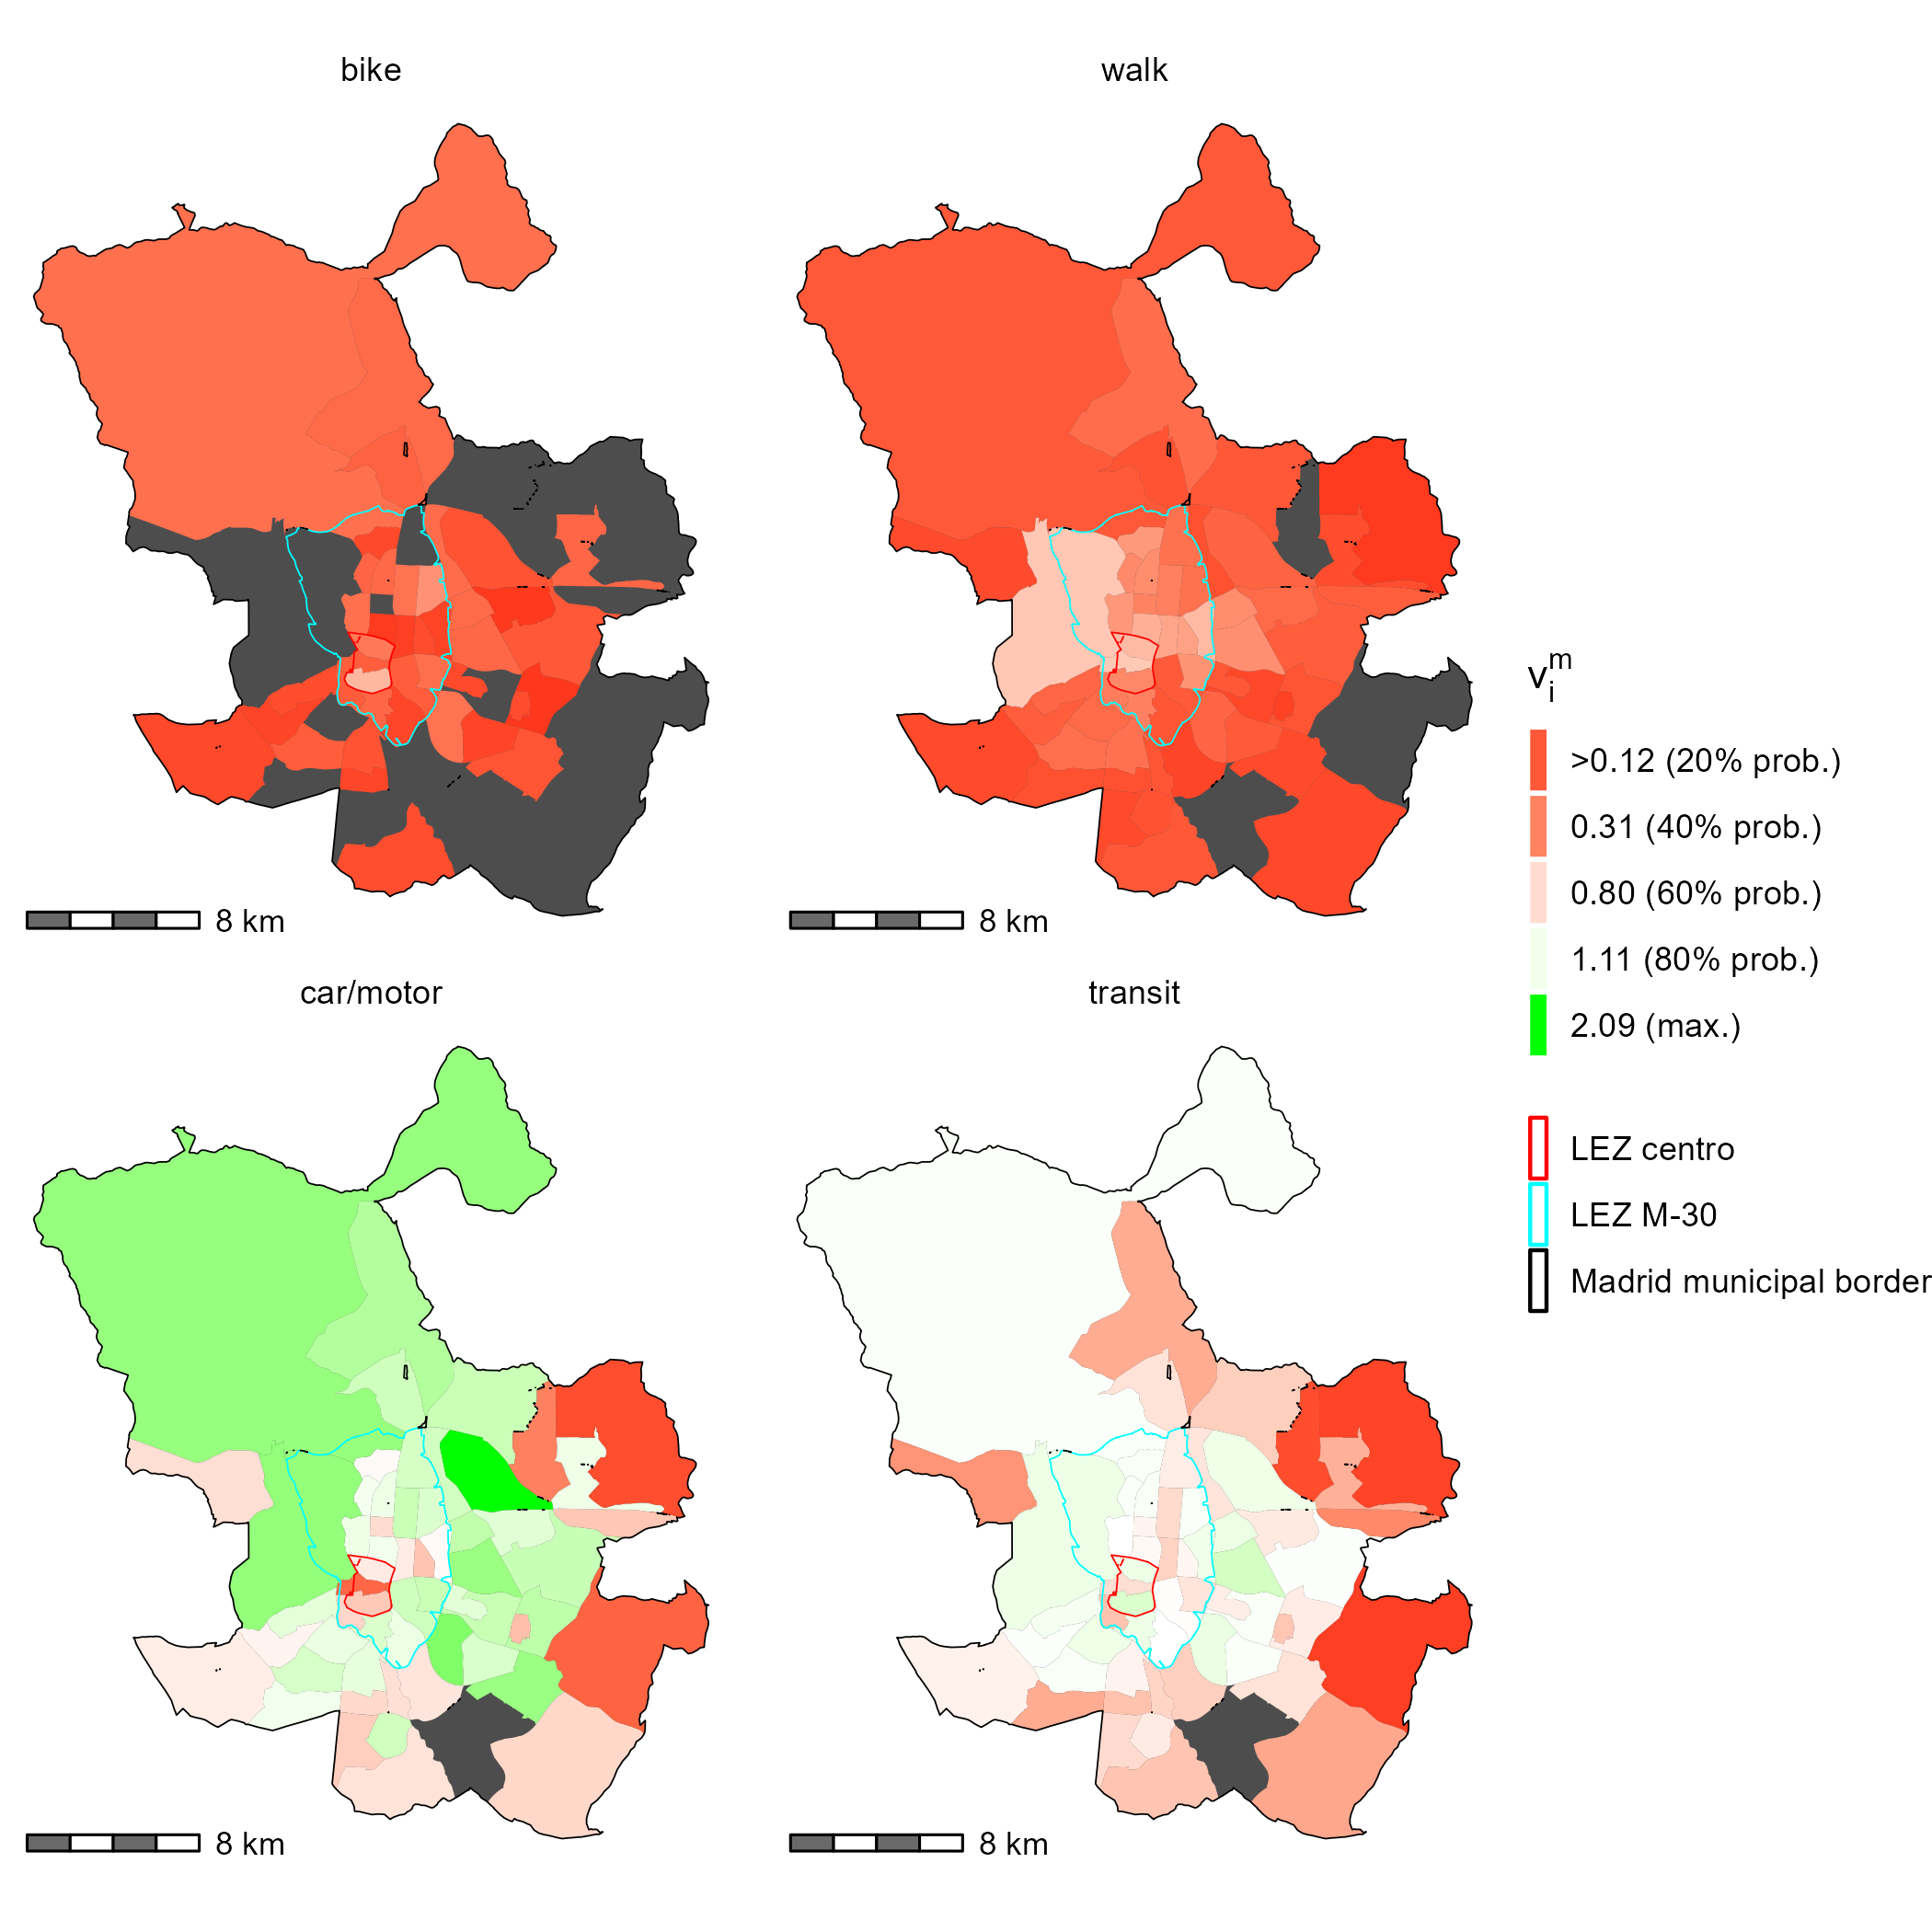
\includegraphics[width=1\linewidth]{images/SA_im_vv_zn208_plot} 

}

\caption{\label{fig:Fig6} Spatial availability of job opportunities per capita per origin and mode $v_i^m$ in Madrid. Calculated using the home-to-work origin destination flows from the 2018 travel survey.}\label{fig:SA-per-capita-m-plot}
\end{figure}

Furthermore, there are spatial differences in the competitive advantage
of spatial availability between modes. Figure \ref{fig:Fig6} visualizes
\(v_i^m\), the spatial availability divided by the mode-population.
These plots illustrates the discussion of the disproportionately high
over-allocation of spatial availability relative to the mode-using
population in many of the origins for the car/motor mode (bottom left
plot, areas denoted with green \(v_i^m\) values above 1). These plots
also visualize areas that disproportionately capture lower spatial
availability (under 1), represented in shades of red. It can be observed
that the transit-using population's spatial availability to jobs is
relatively balanced (i.e., many zones are white), while the
non-motorized modes \(v_i^m\) values are low (under 1).

Interestingly, \(v_i^m\) for car/motor within and near the LEZ Centro is
near or below 1 (white/red): potentially as a consequence, all non-car
modes have relatively higher \(v_i^m\) values in these areas. Though
access to travel survey data immediately before the LEZ implementation
is unavailable, we know that the LEZ Centro shifted more than half of
all car trips into the LEZ to another mode
\citep{tarrinoortizAnalyzingImpactLow2022}. This restriction decreased
the number of car-using population from \(i\)s going into the LEZ Centro
(an area with a large number of jobs - Figure \ref{fig:Fig2}), thus
increasing the mass effect for non-car modes and resulting in
proportionally higher \(v_i^m\) values for non-car modes. Though the
spatial availability from before the LEZ Centro implementation is
unknown, Figure \ref{fig:Fig6} provides a benchmark for quantifying
potential LEZ implementations in the future (given 2018 travel
conditions). Figure \ref{fig:Fig6} also shows that many areas within the
M-30 have high (white/green) \(v_i^m\) values for car-mode, signaling
that the spatial expansion of the LEZ Centro stands to increase the
spatial availability of jobs for non-car mode using populations.

\hypertarget{discussion-and-conclusions}{%
\section{Discussion and conclusions}\label{discussion-and-conclusions}}

Location-based accessibility measures like the Hansen-type \(S_i^m\),
Shen-type \(a_i^m\), and spatial availability \(V_i^m\) measures have a
commonality - they are a weighted sum of opportunities assigned to each
spatial unit \(i\) in a region. How the weight and sum of the
potentially-interacted-with opportunities is considered is what defines
the type of accessibility measure. Within this paper, the location-based
singly- \emph{constrained} and \emph{competitive} accessibility measure,
known as spatial availability \(V_i\)
(\citet{soukhovIntroducingSpatialAvailability2023}), is extended for the
case of capturing multimodal accessibility to opportunities \(V_i^m\). A
synthetic example and then an empirical case of LEZ in Madrid are
detailed to demonstrate this multimodal extension.

The spatial availability measure is capable of capturing a new
interpretation of multimodal competition that previous accessibility
measures have not yet done. Competitive measures hypothesis that
populations using modes with lower travel impedance, when competing for
a finite set of opportunities, will capture more opportunities. With
spatial availability, the number of opportunities that are captured (of
the total opportunities in the region) by each mode can be individually
calculated. From there, the difference between how many spatially
available opportunities one mode captures versus another can be
investigated. This is the advantage of the spatial availability measure,
particularly its multimodal extension.

The flexibility and need for an accessibility measure such as spatial
availability is pertinent in policy scenario evaluation. As showcased in
the empirical example of the LEZ in Madrid, competition for job
opportunity availability varies spatially \emph{as well as} between
modes. The car and transit modes have the highest spatial availability,
with the car mode having highest availability with exception to the
areas within the LEZ Centro. This finding reflects what may suspect are
real conditions: since car travel has been highly restricted within the
LEZ Centro, fewer car-using people potentially interact with jobs within
the LEZ Centro, leaving more \emph{spatially available} jobs for
non-car-using populations. This difference in car-using populations in
locations accessing jobs within and immediately outside the LEZ Centro
increases the competitiveness of the transit-using population (the
second most competitive mode) as well as the non-motorized modes.

Spatial availability \(V_i^m\) can also be divided by the mode-using
population at each \(i\) to yield mode-population normalized values.
These values, reflected in Figure \ref{fig:Fig6}, can be used as a
benchmark to investigate existing conditions and plan future LEZ
implementation (i.e., target areas with exceptionally high car spatial
availability such that more opportunities are available to other
mode-users).

In summary, conventional \emph{non-constrained} accessibility measures
are difficult for planners to operationalize for a variety of reasons
including issues of computation and interpretability
\citep{levinsonTransportAccessManual2020}. With spatial availability,
the magnitude of opportunities that are available as a proportion of all
the opportunities in the region is equal to \(V_i\). As a result of its
proportional allocation mechanism, \(V_i\) can be easily extended into
multimodal applications. This flexibility is pertinent to model policy
scenarios in our cities that are becoming increasingly multimodal. The
interpretation of \(V_i\) allows for manipulation of \(V_i^m\) values to
investigate differences of availability between neighbourhoods, modes,
and regions, generate per capita benchmarks, and/or generate average
values per population-group.

From a spatial equity perspective, spatial availability measure can
provide researchers, policy makers, and citizens a new-found
interpretation of accessibility measures. With a plot of spatial
availability values, one can begin asking, how much is enough and what
level may be too much. These interpretations were difficult to be made
with accessibility measures in the past.

\hypertarget{acknowledgements}{%
\section{Acknowledgements}\label{acknowledgements}}

This research was funded by the Canada Graduate Scholarship - Doctoral
Program (CGS D) provided by the Social Sciences and Humanities Research
Council (SSHRC).

\hypertarget{author-contributions}{%
\section{Author contributions}\label{author-contributions}}

The authors confirm contribution to the paper as follows: study
conception and design: AS, JTO, JSL, AP.; data collection: AS, JTO,
JSL.; analysis and interpretation of results: AS, JTO, JSL, AP.; draft
manuscript preparation: AS, JSL, AP. All authors reviewed the results
and approved the final version of the manuscript.

--\textgreater{}

\newpage
\bibliography{mybibfile.bib}


\end{document}
